% arara: xelatex
% arara: xelatex
% arara: xelatex

% options:
% thesis=B bachelor's thesis
% thesis=M master's thesis
% czech thesis in Czech language
% english thesis in English language
% hidelinks remove colour boxes around hyperlinks

\documentclass[thesis=M,english]{FITthesis}[2012/10/20]

\usepackage[utf8]{inputenc}

\usepackage{graphicx} %graphics files inclusion
% \usepackage{subfig} %subfigures
% \usepackage{amsmath} %advanced maths
% \usepackage{amssymb} %additional math symbols

\usepackage{dirtree} %directory tree visualisation

% ADDED BY ME
%\usepackage{blindtext} % lorem ipsum
%\definecolor{mygray}{gray}{0.6}
%\newcommand{\blind}[1][1]{\textcolor{mygray}{\Blindtext[#1][1]}}

\newcommand{\blind}[1][1]{}

% ALSO ADDED BY ME
\usepackage{todonotes} 


\newcommand{\todotext}[1]{\textcolor{red}{\textbf{[[#1]]}}}
\newcommand{\redtext}[1]{\textcolor{red}{[[#1]]}} 


\setlength{\fboxsep}{0.005pt}
\newcommand{\tmpframe}[1]{\fbox{#1}}
%\renewcommand{\tmpframe}[1]{#1}
\newcommand{\permanentframe}[1]{\fbox{#1}}
\newcommand{\noframe}[1]{#1}


\let\myCite\cite
\renewcommand\cite{\unskip~\myCite}
\let\myRef\ref
\renewcommand\ref{\unskip~\myRef}

% \usepackage{spverbatim} % verb and verbatim with line breaks - doesn't break what I need

\newcommand\hatx{\^{}}
\newcommand{\hatxxx}{\hatx\hatx\hatx}


% list of acronyms
%\usepackage[acronym,nonumberlist,toc,numberedsection=autolabel,nomain]{glossaries}
\iflanguage{czech}{\renewcommand*{\acronymname}{Seznam pou{\v z}it{\' y}ch zkratek}}{}
%\makeglossaries

\newcommand{\tg}{\mathop{\mathrm{tg}}} %cesky tangens
\newcommand{\cotg}{\mathop{\mathrm{cotg}}} %cesky cotangens

% LB
% \setlength{\parskip}{0em}

% % % % % % % % % % % % % % % % % % % % % % % % % % % % % % % % % % % 
% % % % % % % % % % % % % % % % % % % % % % % % % % % % % % % % % % % 
\department{Department of theoretical computer science}
\title{Contextual Shell History}
\authorGN{Šimon} %author's given name/names
\authorFN{Let} %author's surname
\authorWithDegrees{Bc. Šimon Let} %author's name with academic degrees
\author{Šimon Let} %author's name without academic degrees
\supervisor{Ing. Lukáš Bařinka}

\acknowledgements{I would like to thank my supervisor Ing. Lukáš Bařinka for his guidance and advice. His insights and expertise shaped this work significantly. 

Next, my thanks goes to my colleagues and friends for their valuable feedback. They helped me spot my personal biases and assumptions rooted in my personal shell workflows. 

I am grateful for the trust of hundreds of people who downloaded this project. I would also like to thank all GitHub users who submitted issues and pull requests to the project.

I want to thank Installfest conference organizers for the opportunity to give a talk and to demo this project on Installfest.  

Finally, I would like to thank my family for their support during writing this thesis and trough my whole studies.
}
\abstractCS{\todotext{TODO: CZ abstrakt}  \blind[2]}
\abstractEN{\todotext{TODO: abstract} This thesis is an enhancement for standard shell history. It records shell history with context. It uses the recorded context to make it easier to find relevant history records and to make it possible to search search history using context explicitly.

\blind[2]
}
\placeForDeclarationOfAuthenticity{Prague} %where you have signed the declaration
\keywordsCS{Shell, Příkazová řádka, Historie shellu, Nástroje produktivity}
\keywordsEN{Shell, Command line, Shell history, Productivity tools}
\declarationOfAuthenticityOption{1} %select as appropriate, according to the desired license
% \website{https://github.com/curusarn/master-thesis} %optional URL (remove entirely if you have no URL for this thesis) TODO: put the thesis up

\begin{document}

%\newacronym{GUI}{GUI}{Graphical User Interface}
%\newacronym{CLI}{CLI}{Command Line Interface}
%\newacronym{GNU}{GNU}{GNU's Not Unix!}
\begin{introduction}



Classic command line interfaces were mostly replaced by GUIs in consumer software \cite{norman2007ui}. \todo{REF?} However, many professionals around the world still rely on UNIX shells to achieve their daily tasks. CLIs are generally not replaceable by GUIs because GUIs do not scale well when the number of available actions is high \cite{norman2007ui}. 

More than half of all developers use Unix-based operating systems\footnote{According to \cite{stackoverflow2019devsurvey}, 25.6\% and 26.8\% of developers uses Linux and MacOS respectively.}. 
About half of all developers have been working with Linux during year 2018. \cite{stackoverflow2019devsurvey} 

Default shell on GNU/Linux is Bash \cite{ramey1994gnubash} and default shell on MacOS is zsh since October 2019 \cite{apple2019zsh}. In this work we primarily focus on these two popular shells.
\todo{TODO: polish the argument why is this work relevant \hatx\hatx\hatx}

\todotext{TODO: what is the shell history good for}
\todotext{TODO: why could contextual history improve the history offerings}https://www.overleaf.com/project/5d0cfdef69f8f06780064608

The standard shell history contains records with basic information about previously executed command lines. Each record only contains following details: the command line, timedate of the execution, and the duration of the execution\footnote{Duration is only available in Zsh and only when it is enabled.\cite{zshdocs}}. 

Additionally, it is quite common to use shell configuration\footnote{\todotext{e.g. Bash: histocontrol=ignoredups\cite{bashman}; zsh: HIST\_SAVE\_NO\_DUPS\cite{zshdocs}}} to prune duplicates from the history. This removes more information from history because the original command line sequences are lost.

As we can see the standard shell history contains only very basic information about executed command lines.
There is much more contextual data available at the time of command line execution e.g. present working directory, exit status, and previously executed commands. In this work, we explore the possibilities of using the contextual data about executed commands to increase the usefulness of shell history.



% BAD: This limits the potential of standard shell history utilities because shell usage is contextual. is not generally used to run ad-hoc commands but 

% MORE PRACTICAL: When using shells you likely do not run individual commands completely independently of each other. But instead run commands as parts of different workflows that 

\todo{describe the contents of this work / layout - redo because moved chapters in analysis} We start by analysing shell history features to understand advantages and disadvantages of standard shell history. We research existing history tools to see what ideas were already explored, which features work and which do not. 

After that, we focus on people. We start broad and research how people use computer tools in general. Then we move on to examining how people use shell and shell history. We also look at public discourse related to history tools and engage in online discussions to find out more about configurations and tools people use.

Next, we focus on the contextual information; We cover what information is available to be saved at the time of command line execution and we discuss how it could be used to enhance shell history. 

At this point we move on to design(ing) ...
\todotext{TODO: finish this intro}


\blind[2]

\end{introduction}


% \begin{verbatim}
% ____5___10___15___20___25___30___35___40___45___50___55___60__64
% \end{verbatim}
% The page is 64 verbatim characters wide

\todo{GLOBAL TODOs}

\todo{REPLACE: users -$>$ people (where suitable)}
\todo{TODO: use singular they ??? - REPLACE: the user, he -$>$ the user, they}
\todo{REPLACE "command line" -$>$ "command line entry" / "command line submission" / "history entry"}
\todo{REPLACE "command" -$>$ "command stub" / "stub"}
\todo{REPLACE "bash" -$>$ "Bash"}
\todo{REPLACE "zsh" -$>$ "Zsh"}
\todo{REPLACE other shells -$>$ Capitalize}
\todo{CHECK if verbatims are not split between pages in a weird way}

\todo{SPELLCHECK: grammarly}
\todo{SPELLCHECK: ask Sue}

\todo{CONSISTENCY: CTRl-P vs CTRL+P}


% every \permanentframe shout have 0.995 img size



\chapter{Analysis}

\todo{DEFINE "command line entry"/"history entry" is a full command entered/submitted by the user}
\todo{DEFINE "stub"/"command stub" is the first word of the command line entry - usually an executable, a shell builtin, or an alias.}



\todotext{TODO: describe layout/contents of the chapter}

\blind

\section{Origins of standard history features in shells}

In this chapter we explore the standard shell history features which are most likely available to majority our target users.
Most of the history features we see and use today were adopted from older shells. Many of these features stayed similar to their original versions. We look at the shells and the history features chronologically to see the evolution and improvements in shell history facilities over the years.  


\begin{figure}
  \tmpframe{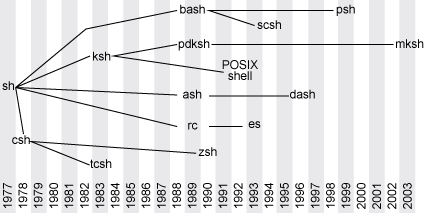
\includegraphics[width=\linewidth]{figures/misc/shells.png}}
  \caption{Linux shells since 1977, from \cite{jones2011shells} \todotext{TODO: Better quality or begone.}}
\end{figure}

\todotext{TODO: Add summaries of the features using bullet point lists.}
\todotext{TODO: Point out drawback of the features as you describe them.}
\todotext{TODO: Break up the walls of text with bold text and bullet point lists.}

\subsection{History features of C shell}

C shell (Csh) was initially released in 1978. 
It features history substitution: a simple history mechanism enabling reuse of previously executed commands inspired by Interlisp\cite{joy1994cshintroduction}. Size of the history is configurable\footnote{Examples featured in \cite{joy1994cshintroduction} and \cite{dubois1995tcshusing}
show history size set to 10 and 20 records respectively.} but according to \cite{cshman}, too large values may run the shell out of memory.

% History is disabled by default (I think) persistence accross sessions is on my install

C shell history substitution allows the user to reuse: the previous command line using \verb|!!|, the last argument of the previous command line using \verb|!$|, and all arguments of the previous command line using \verb|!*|. To run other commands lines than the previous one we could use \verb|!cc| which executes the last command line from history starting with \verb|cc|. Executing a command line based on absolute or relative index can be done using \verb|!5| or \verb|!-2| respectively. To see what command is about to be executed we could use e.g. \verb|!cc:p|, \verb|!5:p|, or \verb|!-2:p|; This only prints the history record instead of executing it. It is also possible to replace parts of command lines using \verb|!!:s/foo/bar/| or a shorthand \verb|^foo^bar| where \verb|foo| is replaced by \verb|bar| in the previous command and the result gets executed. \redtext{When using these features we do not see the resulting substituted command line until executing it. This can lead to errors or printing the substitutions first which slows users down.}
    
There is a \verb|history| command which prints out recent history records with their indexes. There are also other less notable history substitution features available; These are accessible using different modifiers that can follow \verb|!| character. Another noteworthy features of Csh are: file name tab completion, tilde expansion, command aliases, and job control.\todo{check \& ref? } \redtext{history can be easily persisted across logins}

\redtext{savehist - allows to merge history instead of overwriting it}
%savehist
%If set, the shell does 'history -S' before exiting. If the first word is set to a number, at most that many lines are saved. (The number must be less than or equal to history.) If the second word is set to 'merge', the history list is merged with the existing history file instead of replacing it (if there is one) and sorted by time stamp and the most recent events are retained. (+)
\redtext{commands lines are saved to history after the history expansion is performed}


\subsection{History features of Tenex C shell}
Tenex C shell (Tcsh) is an enhanced version of the C shell released in 1983\todo{REF}; It offers command line editing and programmable tab completion\cite{dubois1995tcshusing}. Since Tcsh is a version of C shell, it does support all the previously described features of C shell. The history holds 100 previous command lines by default and it also contains datetime of the command line execution.

Tcsh offers command line editing; This means that the user can manipulate the contents of the command line by using various built-in functions. A few examples of such functions are: \verb|delete-word|, \verb|expand-glob|, and \verb|history-search-backward|. All built-in functions can be bound to arbitrary key combinations. Additionally, Tcsh features emacs and vi editing modes which come with default keybindings usual for the respective editors. When describing the default keybindings for Tcsh in this section we are only considering the emacs mode.

A portion of built-in functions allows the user to reuse command lines from the shell history. Functions \verb|up-history| and \verb|down-history| allow the user to step through the history; Default keybindings are \verb|CTRL-P| and \verb|arrow_up| for \verb|up-history|; and \verb|CTRL-N| and \verb|arrow_down| for  \verb|down-history| \cite{tcshman}. This is something you are likely already used to in your modern shell.

% BAD ALT: Pressing \verb|CTRL-P| invokes \verb|up-history| function which replaces the current command line contents with previous command line from history. Pressing \verb|CTRL-P| repeatedly continues up through the history. Pressing \verb|CTRL-N| invokes \verb|down-history| function which steps through the history in the other direction. These two functions are also often bound to \verb|arrow_up| and \verb|arrow_down| keys. 

Besides stepping through history, Tcsh features prefix search. The functions \verb|history-search-backward| \todo{make sure this doesn't overflow :( } and \verb|history-search-forward| use the command line contents before the cursor as a prefix to search the history in the desired direction. The default keybindings for these functions are a little weird; \todo{TODO: Pressing ESC an then x is just a way of pressing ALT-x without having ALT. }
You need to press \verb|ESC| and then \verb|p| or \verb|n| for backward or forward search respectively. 

Another useful history feature of Tcsh is interactive string search. In contrast to prefix search this feature allows us to search history using any part of the command line not just the prefix. This feature is realised by \verb|i-search-back| and \verb|i-search-fwd| functions. Invoking these functions prints a secondary prompt under the primary one: \verb|bck:| or \verb|fwd:| depending on the invoked function. Typing searches the history interactively in the desired direction. Invoking the functions repeatedly steps through the history records that match the query.
These functions sound quite useful but despite that they are not bound to any keys by default.
% \redtext{So the users need to set up the key bindings themselves.}

Activating vi mode in Tcsh changes some of the keybindings. In addition to regular keybindings, stepping through history is available on keys \verb|K| and \verb|J|, and prefix search is available on \verb|SHIFT-K| and \verb|SHIFT-J|. Instead of \verb|i-search-back| and \verb|i-search-fwd| functions vi mode offers \verb|vi-search-back| and \verb|vi-search-fwd| with similar functionality.
% \redtext{vi mode has defaults - back: ? ,fwd: /}

\redtext{histdup - prunes duplicates from history}
% tcsh man page (+ means "not available in csh")
%histdup (+)
%               Controls  handling  of  duplicate  entries in the history list.  If set to `all' only unique history events are entered in the history list.  If set to `prev' and the last
%               history event is the same as the current command, then the current command is not entered in the history.  If set to `erase' and the same event is  found  in  the  history
%               list, that old event gets erased and the current one gets inserted.  Note that the `prev' and `all' options renumber history events so there are no gaps.


% Since we are mainly interested in history features we only focus on the functions that use history 
% Command line editing was an important step forward in interactive shell use. It enables the user
% As the name suggest it was inspired by features available in Tenex operating system. 

\subsection{History features of Korn shell}
Korn shell (Ksh) was initially released in 1983; It was originally written as a proprietary software until being released as open source in 2005. \todo{REF} History features of Korn shell are a very similar to the features of Tenex C shell. Ksh offers stepping through history, string search, and vi mode variant of the string search. It is worth mentioning that in Ksh, string search is bound to \verb|CTRL-R| by default which is what you are probably used to in modern shells. 

Ksh offers a shell builtin command \verb|fc| that provides a superset of C shell history mechanism\cite{rosenblatt2000kshlearning}. It allows the user to list recent history entries, edit command lines from history with an editor, and run history entries with changes. Running \verb|fc -l| lists the previous command lines from history (with indexes). So does \verb|history|, because in Ksh it is just an alias for \verb|fc -l|. To edit previous command line from history in an editor we could use \verb|fc| (without arguments) which executes the resulting command after we are done editing it. If we want to choose an editor we could use \verb|fc -e vi|. Running \verb|fc -e - foo=bar| skips the editing, replaces occurrences of \verb|foo| with \verb|bar| and executes the result. To access more then the previous command line we would use absolute or relative indexes similarly to the history expansion in Csh. For example, \verb|fc 5| and \verb|fc -2| opens an editor with fifth from the history list and the second command relative to current command line. It is also possible to select ranges of commands for editing with e.g. \verb|fc -2 -6|.

% We are not describing other Ksh history features in detail because of the similarity with already described Tcsh history features.


\subsection{History features of Bourne again shell}
Bourne again shell (Bash) was initially released in 1989.
Default history size in Bash is 500 records.\cite{bashman} Each history entry contains datetime of the execution. Unless the user disables the \verb|cmdhist| option, all lines of a multi-line command are saved as one history record; Based on \verb|lithist| option, newlines are either embeded into history or replaced by semicolons to keep the syntax of the saved commands correct. 

There are shell variables that can be used to prevent certain command lines from being saved to history. Variable \verb|HISTCONTROL| can be used to prevent saving duplicates, and to skip saving command lines starting with a space. Variable \verb|HISTIGNORE| allows using pattern matching to prevent various command lines from being saved into history.  

Bash features history expansion (\verb|!!|, \verb|!$|, \verb|!cc|, etc.) which is compatible with the Csh\cite{ramey1994gnubash}.
Bash features a \verb|histverify| option that alters the behaviour of history expansion. When it is enabled, the results of history expansion are  pasted onto the command line instead of being executed immediately. This option is disabled by default. 

\todo{COMMENTED: use this later as an example for memory load}
% It seems that authors of Bash realised the danger of history expansion; It forced the users were either forced to rely on their memory or to explicitly ask for the history expansion result to be printed first.}
% This shows us both the importance of not relying on memory/recall and the importance of adhering to the existing standard.
\todo{NOTE: we could briefly introduce Readline}
Command line editing in Bash provides most of the history related functions from Tcsh. Some of these functions have different names and some of them have different default keybindings.

Functions for stepping through history \verb|up-history| and \verb|down-history| are named \verb|previous-history| and \verb|next-history| respectively; Default keybindings did not change. 

Interactive string search (better known as reverse search) is available in Bash as \verb|reverse-search-history| and \verb|forward-search-history| with default keybindings \verb|CTRL-R| and \verb|CTRL-S|. 
Common issue with this keybinding is that \verb|CTRL-S| is often used to freeze the output of the terminal using OS's terminal driver\todo{REF: ask Barinka, he will know}; This means that many users do not have the option to search in the "forward" direction.   
Bash also provides non-interactive versions of these functions bound to \verb|ALT-P| and \verb|ALT-N|. However, besides saving your CPU from searching the history multiple time, they do not seem to provide any advantage over their interactive counterparts. 

Prefix search functions are still available under the same name (\verb|history-search-backward| \todo{overflow!} and \verb|history-search-forward|) but they do not have default keybindings in Bash. Alternative substring searching versions for these functions are available which do not search just by prefix but can match anywhere on the command line: \verb|history-substring-search-backward| and \verb|history-substring-search-forward|.\todo{overflow!}

Another two history functions we can find in Bash are \verb|yank-last-arg| and \verb|yank-nth-arg|. The first one pastes the last argument of the previous history entry onto the command line. The second one pastes the Nth argument. Default keybindings for \verb|yank-last-arg| are \verb|ALT-.| or \verb|ALT-_|. To use \verb|yank-nth-arg| we need to provide an argument to Bash input library; This can be done by pressing an \verb|ALT| key with a numeric argument. Then we can press \verb|CTRL-ALT-Y|. Without providing any argument the function pastes the first argument of the previous history entry onto the command line.


Other than command line editing functions Bash offers builtin commands to list, reuse and manipulate the history. The \verb|fc| builtin is very similar to the one available in Ksh. We can list of recent command lines from history with \verb|fc -l|, edit and execute them with \verb|fc| without any arguments, and substitute and execute them with \verb|fc -s foo=bar|. It is possible to select command lines and ranges of command lines from the history using absolute or relative indexes.

Compared to Ksh, \verb|history| is no longer just an alias; It is a Bash builtin which can be used to display and control the shell history. Without any arguments, \verb|history| prints out a list of previous history entries with indexes. Using various command line options it can be used to: add command lines to history, delete them, or clear the history. It can load new or all history entries from the history file to the history of this shell session; New entries could appear in the history file because of other simultaneously running shell sessions. Conversely, we can use the \verb|history| builtin to append or write the history of this shell session to the history file.


\subsection{History features of Z shell}

Z shell (Zsh) was originally released in 1990. Most of the history features available in Bash are also offered by Zsh.
The default history size is just 30 lines. The history contains the executed command line, the datetime and the duration of the execution. This information is only saved to history when the \verb|EXTENDED_HISTORY| option is enabled. 

% Zsh is overall more feature-rich than Bash. 
% Many features and options that are natively supported in Zsh are non-trivial or impossible to set up in Bash\todo{example?, ref?}.
% We are not going to cover Zsh in great detail because of its similarity to Bash.

Zsh does feature csh-style history expansion. Like Bash, it can be configured to evaluate the history expansion and paste the result onto the command line instead of executing it; This behavior can be enabled using \verb|HIST_VERIFY| option. Another way to see what the history expansion evaluates to is the \verb|magic-space| function. It evaluates history expansion and inserts a space when invoked. When we bind this function to spacebar the history expansion will get evaluated every time we press \verb|SPACE|.

\todo{NOTE: we could briefly introduce ZSH ZLE}
We can find Zsh equivalents for almost all Bash command line editing functions that allow history reuse. In addition, we can find variations and extra functions compared to what is available in Bash. Using \verb|arrow_up| and \verb|arrow_down| keys we can retrieve recent command lines from history. Prefix search is available but unbound by default. There is a variant of prefix search that always searches by first word on the current command line no matter where the cursor is. This variant of prefix search is bound to \verb|ALT-P| and \verb|ALT-N| by default. Interactive reverse search functions are also available with the same default keybindings as in Bash.

Zsh offers pattern matching variants for the most of the history searching functions; These treat the typed query as a pattern instead of a string that should be matched exactly. Vi mode variants for some of the searching functions are available as well.  

The \verb|fc| builtin command is supported and the functionality is comparable to its Bash counterpart. Like in Ksh, \verb|history| is just an alias for \verb|fc -l|. 

% There are alternatives to achieve almost anything that can be done in Bash. For example, ...


\blind
\todotext{TODO: short conclusion about shells ? }


\section{How people use shell}

In this chapter we examine how people use shell and shell history. We consider previous research that studies the properties of how people use command based systems. We also collected a sample of user shell histories and we will be discussing where our data matches the existing findings and where it does not. 

We are looking at properties of command line usage to see if find justifications for standard history features. Examining shell history could also give us insights into how to design history tools. 

After examining shell usage itself we focus on how people use shell history features. We explore existing online discourse about history tools to discover common workflows, problems and configurations.

\subsection{Collecting shell history}

\todotext{TODO: describe how we collected history (skipping errors)}
\blind

\subsection{Frequency distributions of commands}

In this section, we focus on commands instead of whole command lines. By command we mean the first word of the command line executed by the user. Command is usually an executable program or a shell builtin.

\redtext{According to \cite{greenberg1993computer}, frequency distribution of commands used by a group of similar users follows Zipf distribution.}

\redtext{Zipf distribution has the property that a relatively small number of items have high usage frequencies, and a very large number of items have low usage frequencies.}

\todotext{TODO: 80-20 rule is a looser characteristic of Zipf distribution - 20 \% of items account for 80 \% of usage ... alternative 90-10}
\blind
80-20 rule -$>$ https://en.wikipedia.org/wiki/Pareto\_principle



\todotext{TODO: describe and explain the plots}

% A looser characteristic of this kind of rank distribution is the well-known 80-20 rule of thumb that has been commonly observed in commercial transaction systems - 20\% of the items in question are used 80\% of the time (Knuth, 1973; Peachey,Bunt, and Colbourn, 1982).2

% In measurements recorded from a UNIX site, Hanson, Kraut, and Farber (1984) report a similar trend - 10\% of the 400-500 commands available account for 90\% of the usage


% Figure 3.1. The normalized command frequency, compared with Zipf.

\begin{figure}
  \tmpframe{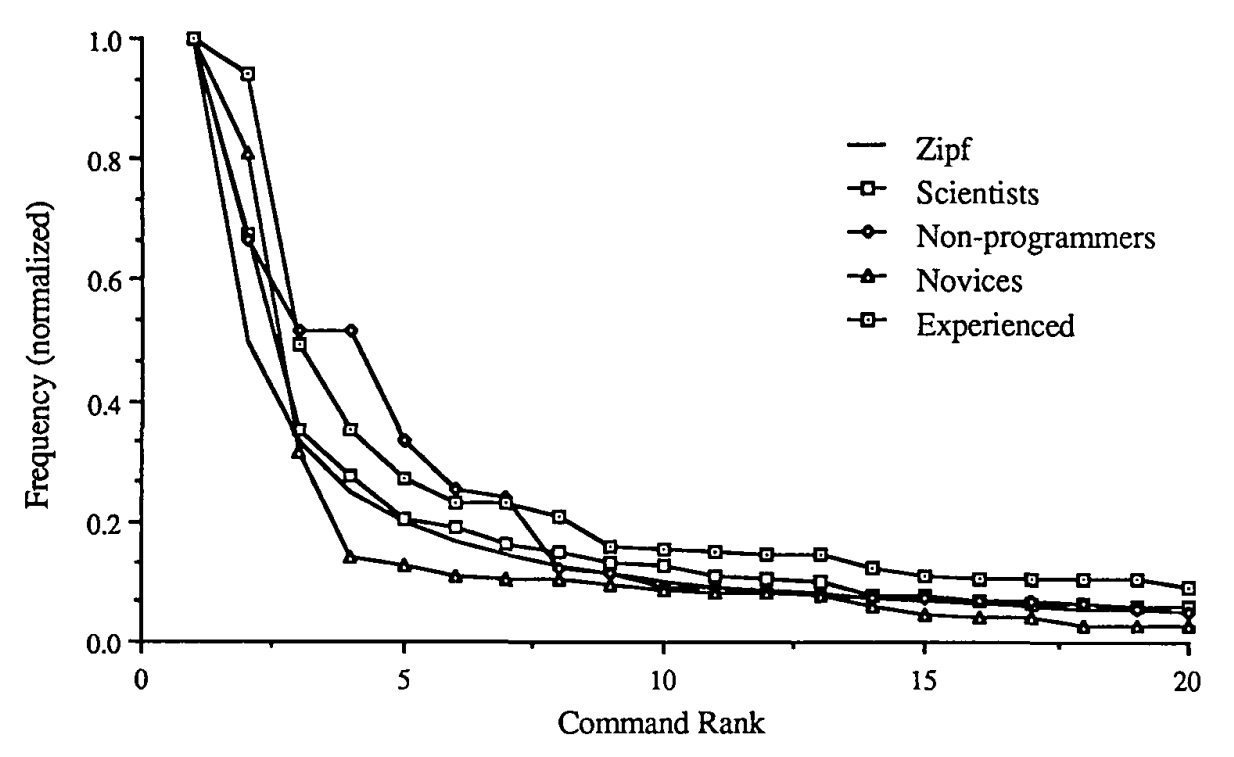
\includegraphics[width=\linewidth]{figures/greenberg/plot_ref_zipf-cmd-frq.png}}
  \caption{The normalized command frequency, compared with Zipf from \cite{greenberg1993computer}}
\end{figure}

\begin{figure}
  \tmpframe{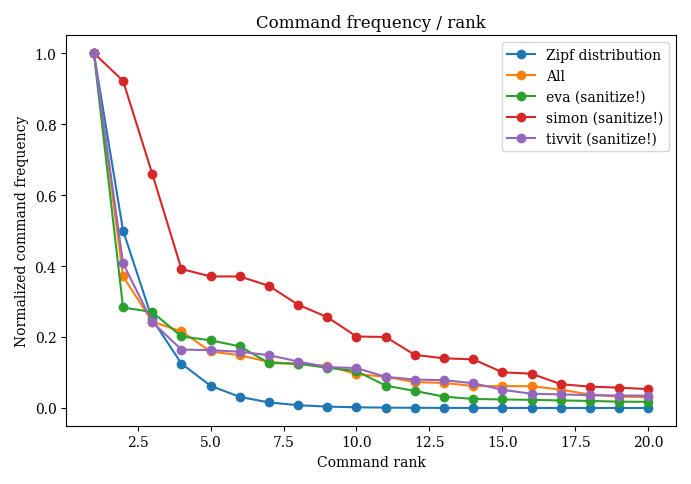
\includegraphics[width=\linewidth]{figures/greenberg_new/plot_zipf-cmd-frq.png}}
  \caption{The normalized command frequency, compared with Zipf. \todotext{unify labels to match Greenberg, export in vector, lose top title, add data from more people}}
\end{figure}
\todo{command rank plots should be on the same page}
\todo{make sure figures are not all over the place}

\todotext{TODO: In our plot the combined history of all the subjects somewhat follows zipf. BUT also most of the individual users follow the zipf - there are exceptions. In Greenberg study individual histories did not follow zipf.}

% ALL: Top 100 %% of cmds amounts for 100.0 %% of all command lines
% ALL: Top 10 %% of cmds amounts for 63.43728659230594 %% of all command lines
% ALL: Top 20 %% of cmds amounts for 71.34987480081949 %% of all command lines
% eva: Top 100 %% of cmds amounts for 100.0 %% of all command lines
% eva: Top 10 %% of cmds amounts for 62.012411347517734 %% of all command lines
% eva: Top 20 %% of cmds amounts for 73.35992907801419 %% of all command lines
% simon: Top 100 %% of cmds amounts for 100.0 %% of all command lines
% simon: Top 10 %% of cmds amounts for 57.7319587628866 %% of all command lines
% simon: Top 20 %% of cmds amounts for 66.18556701030928 %% of all command lines
% tivvit: Top 100 %% of cmds amounts for 100.0 %% of all command lines
% tivvit: Top 10 %% of cmds amounts for 53.33086145099493 %% of all command lines
% tivvit: Top 20 %% of cmds amounts for 64.93634902978619 %% of all command lines


\todotext{TODO: According to \cite{greenberg1993computer},: For each of the four
user groups, 10\% of the commands used accounted for 84\%-91\% of all usage}


\redtext{Top 10 \% of cmds amounts for 63 \% of all command lines}
\redtext{Top 20 \% of cmds amounts for 71 \% of all command lines}

\redtext{Our data does somewhat follow the 80-20 (71-20) rule (relatively few items account for a significant portion of the distribution) but it is a significant difference compared to the stats from the study. Because of the low number of subjects we can only theoretize why this is - more commands available?, small sample size?, longer collection period?}

\redtext{We suspect that difference is mainly caused by larger number of commands used by the users overall}

\redtext{TODO: Top used commands differ between people}
\redtext{According to greenberg, even when people have very similar expertise and identical goals the commands they use vary significantly. Surprising number of commands is not shared by the users from the same group. This diversion shows that there are many ways to achieve the same goal. Commands are smaller units that make up the goals of the users. - Our data is in line with these ideas.} 

\todotext{Conclusion: Command frequencies are highly uneven and individual.}

\subsection{Command Vocabulary}

\redtext{Command vocabulary is the set of commands used by a given person. We are interested in analysing how the vocabulary of the user changes over time.}

\todotext{TODO: describe and explain plots}


% Figure 3.2. Command vocabulary size vs. the number of command lines entered for four individuals.

\begin{figure}
\centering
  \tmpframe{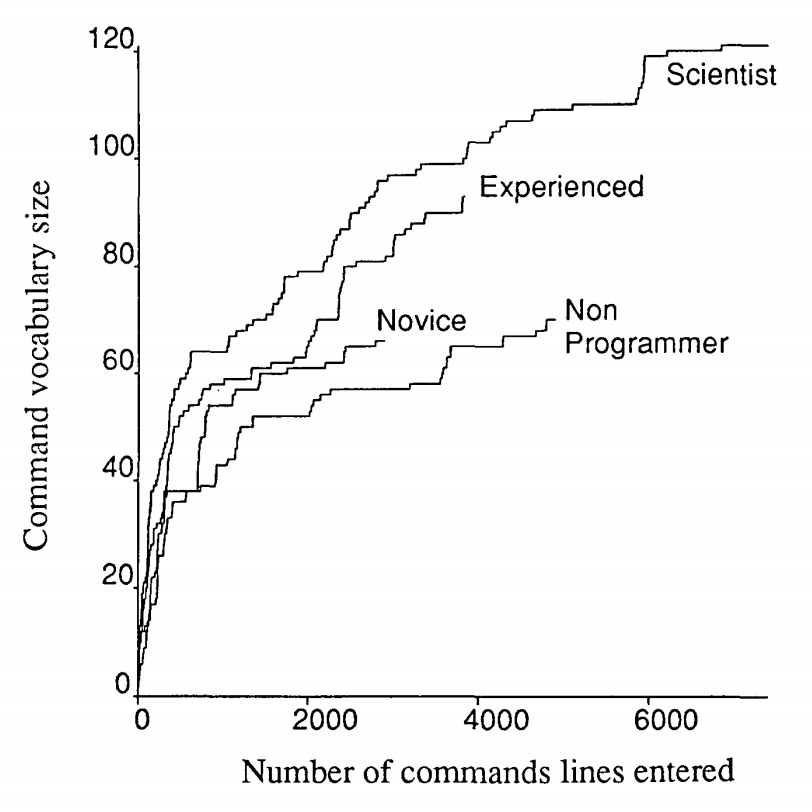
\includegraphics[width=0.6\linewidth]{figures/greenberg/plot_ref_cmd-vocab-size.png}}
  \caption{Command vocabulary size vs. the number of command
lines entered for four individuals. (Greenberg)}
\end{figure}

\begin{figure}
  \tmpframe{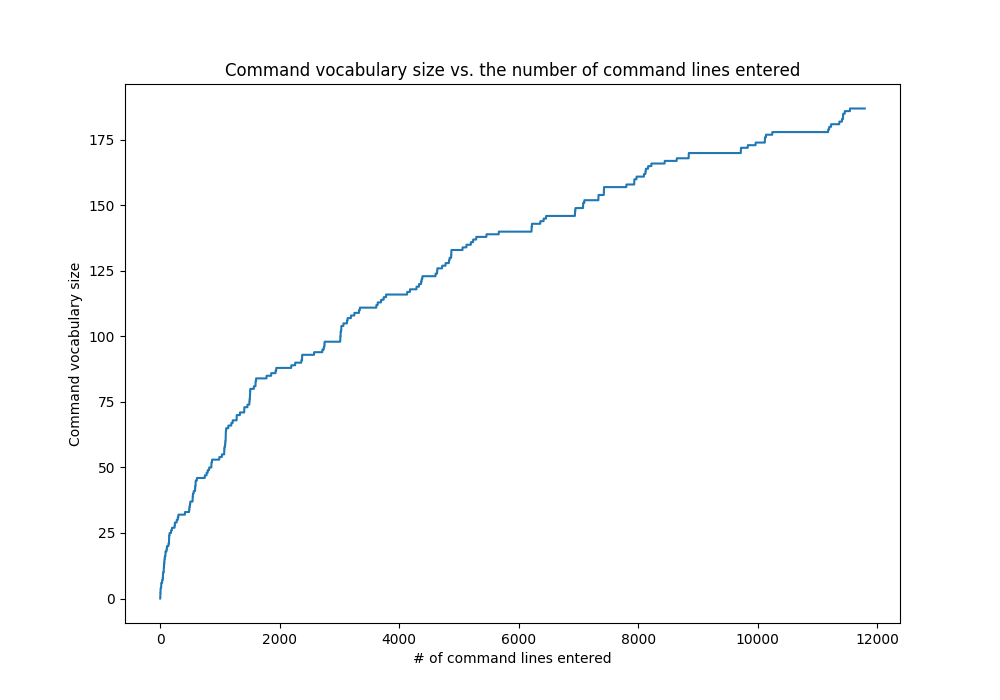
\includegraphics[width=\linewidth]{figures/greenberg_new/plot_cmd-vocab-size.png}}
  \caption{Command vocabulary size vs. the number of command
lines entered for \todotext{N individuals}}
\end{figure}

\begin{figure}
  \tmpframe{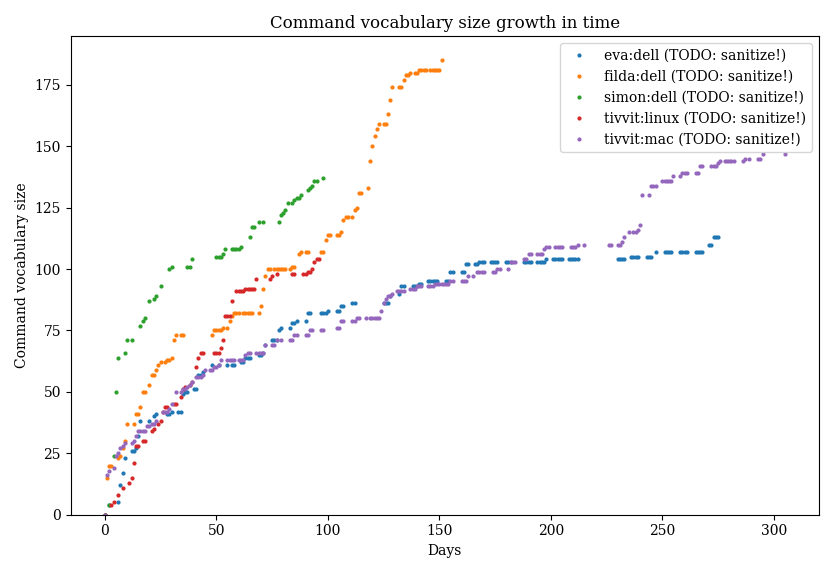
\includegraphics[width=\linewidth]{figures/greenberg_new/plot_cmd-vocab-size-time.png}}
  \caption{Command vocabulary size in time of \todotext{N individuals} (empty spaces are for days without any shell history)}
\end{figure}




\todotext{TODO: initial "steep" period in the plot is caused by the system encountering the commands for the first time. the more stable part is more representative of actual adoption rate of new commands.}

\todotext{TODO: Greenberg found out that bursts in adoption of new commands is sometimes caused by new goals of the user but sometimes no such new goal can be found in the data. Our data does support this. }

\redtext{Greenberg reports adoption or about 5\% for all users before they enter 1k command line. He concludes that this is an initial learning period when the system encounters most of the commands for the first time. According to Greenbers, after initial 1k cmd lines entered the adoption rate drops quicky under 1\%. This is somewhat in line with our findings. We did observe about 5\% cmd adoption rate during the first 1k cmdlines entered for vast majority of our users. Between 1k and 2k we saw a drop in adoption of new commands to about 3\%. After 2k the adoption dropped to numbers lower than 2\% for most users.}

\todotext{TODO: Two differences - longer initial period of 2k cmdlines and higher adoption rate of up to 2\%}

\redtext{These differences could be caused by multiple factors. There is more commands available compared to XX years before. Additionally, custom commands/scripts seem to be quite common in our data while they seem to be non-existent in the greenberg study. This alone could have a huge impact. Draper (see below) was referring to a number of commands available to users of ... as 570. }

\redtext{Nowadays the number of available commands is virtually unlimited because users can install and create new commands. Number of initially available commands on a newly installed system is in thousands.}

% REF: Draper (1984) estimated the times a command was invoked by noting the UNIX processes spawned during each user's interaction with the system (method 4, Section 2.2.1).5 He suggested that the overall trends observed are representative of real command use. First, out of a vocabulary of the 570 commands available to the population, only 394 (70\%) were used at least once. 

\redtext{We can conclude that command usage distribution was and still is very uneven (few commands dominate the distribution) and that the number of available commands slowly and unevenly increases over time but the adoption of new commands is faster than in the past.}

\redtext{new workflows, aliases, ...}

% eva: Cmd adoption rate at 1k (between 0 and 1k) cmdlines = 0.051
% eva: Cmd adoption rate at 2k cmdlines = 0.0345
% eva: Cmd adoption rate between 1k and 2k cmdlines = 0.018
% eva: Cmd adoption rate between 2k and 3k cmdlines = 0.013
% eva: New cmd adoption rate after 1k cmdlines = 0.007725856697819315
% eva: New cmd adoption rate after 2k cmdlines = 0.006263345195729538
% eva: New cmd adoption rate after 3k cmdlines = 0.005145228215767635
% simon: Cmd adoption rate at 1k (between 0 and 1k) cmdlines = 0.076
% simon: Cmd adoption rate at 2k cmdlines = 0.0505
% simon: Cmd adoption rate between 1k and 2k cmdlines = 0.025
% simon: Cmd adoption rate between 2k and 3k cmdlines = 0.007
% simon: New cmd adoption rate after 1k cmdlines = 0.015840041547649963
% simon: New cmd adoption rate after 2k cmdlines = 0.012627148368993335
% simon: New cmd adoption rate after 3k cmdlines = 0.015667206915180983
% tivvit: Cmd adoption rate at 1k (between 0 and 1k) cmdlines = 0.045
% tivvit: Cmd adoption rate at 2k cmdlines = 0.0315
% tivvit: Cmd adoption rate between 1k and 2k cmdlines = 0.018
% tivvit: Cmd adoption rate between 2k and 3k cmdlines = 0.011
% tivvit: New cmd adoption rate after 1k cmdlines = 0.009304948540814888
% tivvit: New cmd adoption rate after 2k cmdlines = 0.007877892663712457
% tivvit: New cmd adoption rate after 3k cmdlines = 0.007264873355586099
% >>> Avg recurrence rate = 70.29523637022278
% >>> Max avg recalled characters = 16.34658576344865
% >>> Max avg recalled characters (including prefix matches) = 26.770874841514217

\subsection{Sequential dependencies between commands}

We just looked at frequencies of commands and command vocabulary of shell users. Now we take a look the dependencies between commands.

\todotext{TODO: describe the graph by Hanson - all users together, node size indicates frequency of the command, arrows indicate significant dependencies, 50 cmds. }

\todotext{TODO: describe findings by Hanson - significant chains, core/modular cmds vs. cmds with significant dependencies, functional clusters of commands}



% Figure 3.3. Sequential structure of UNIX command usage, from Figure 4 in Hanson et al. (1984).

\begin{figure}
  \tmpframe{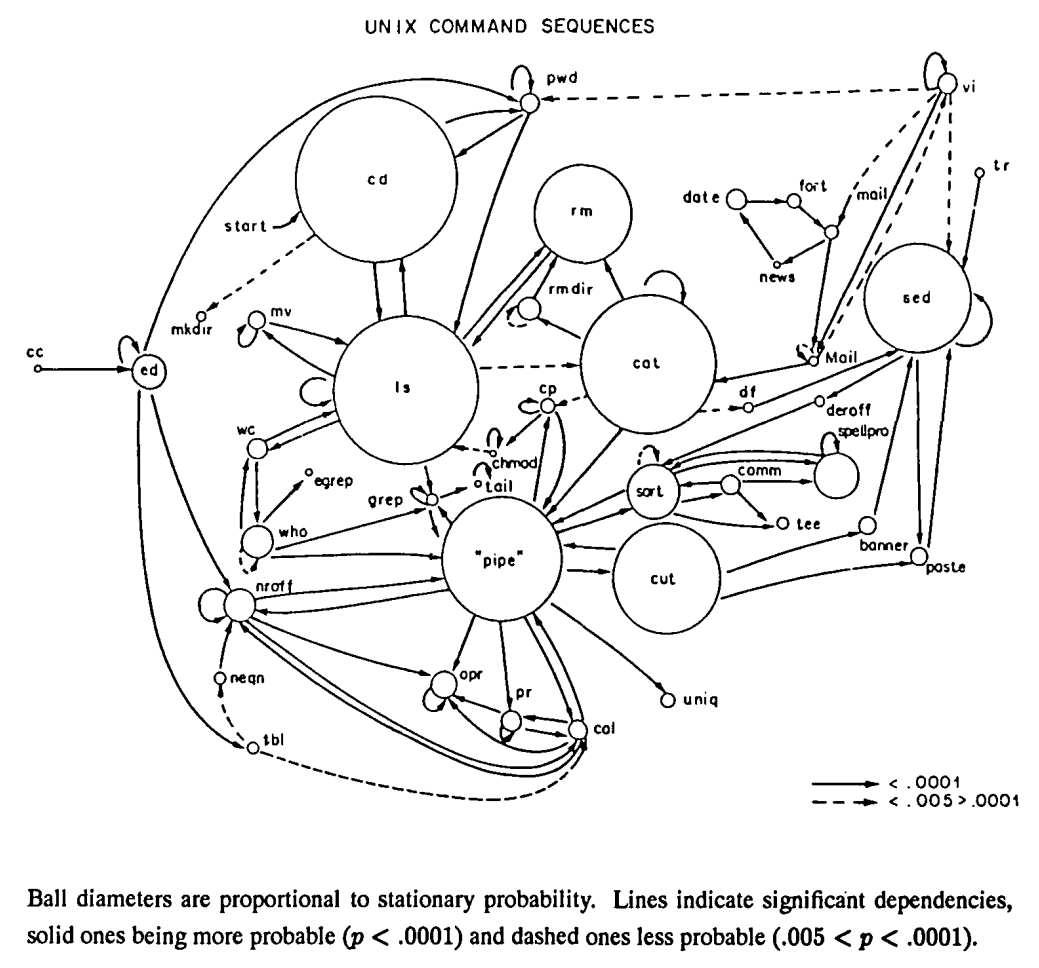
\includegraphics[width=\linewidth]{figures/greenberg/graph_ref_cmd-sequences.png}}
  \caption{Sequential structure of UNIX command usage, from Figure 4
in Hanson et al. (1984). (Greenberg)}
\end{figure}

\begin{figure}
  \tmpframe{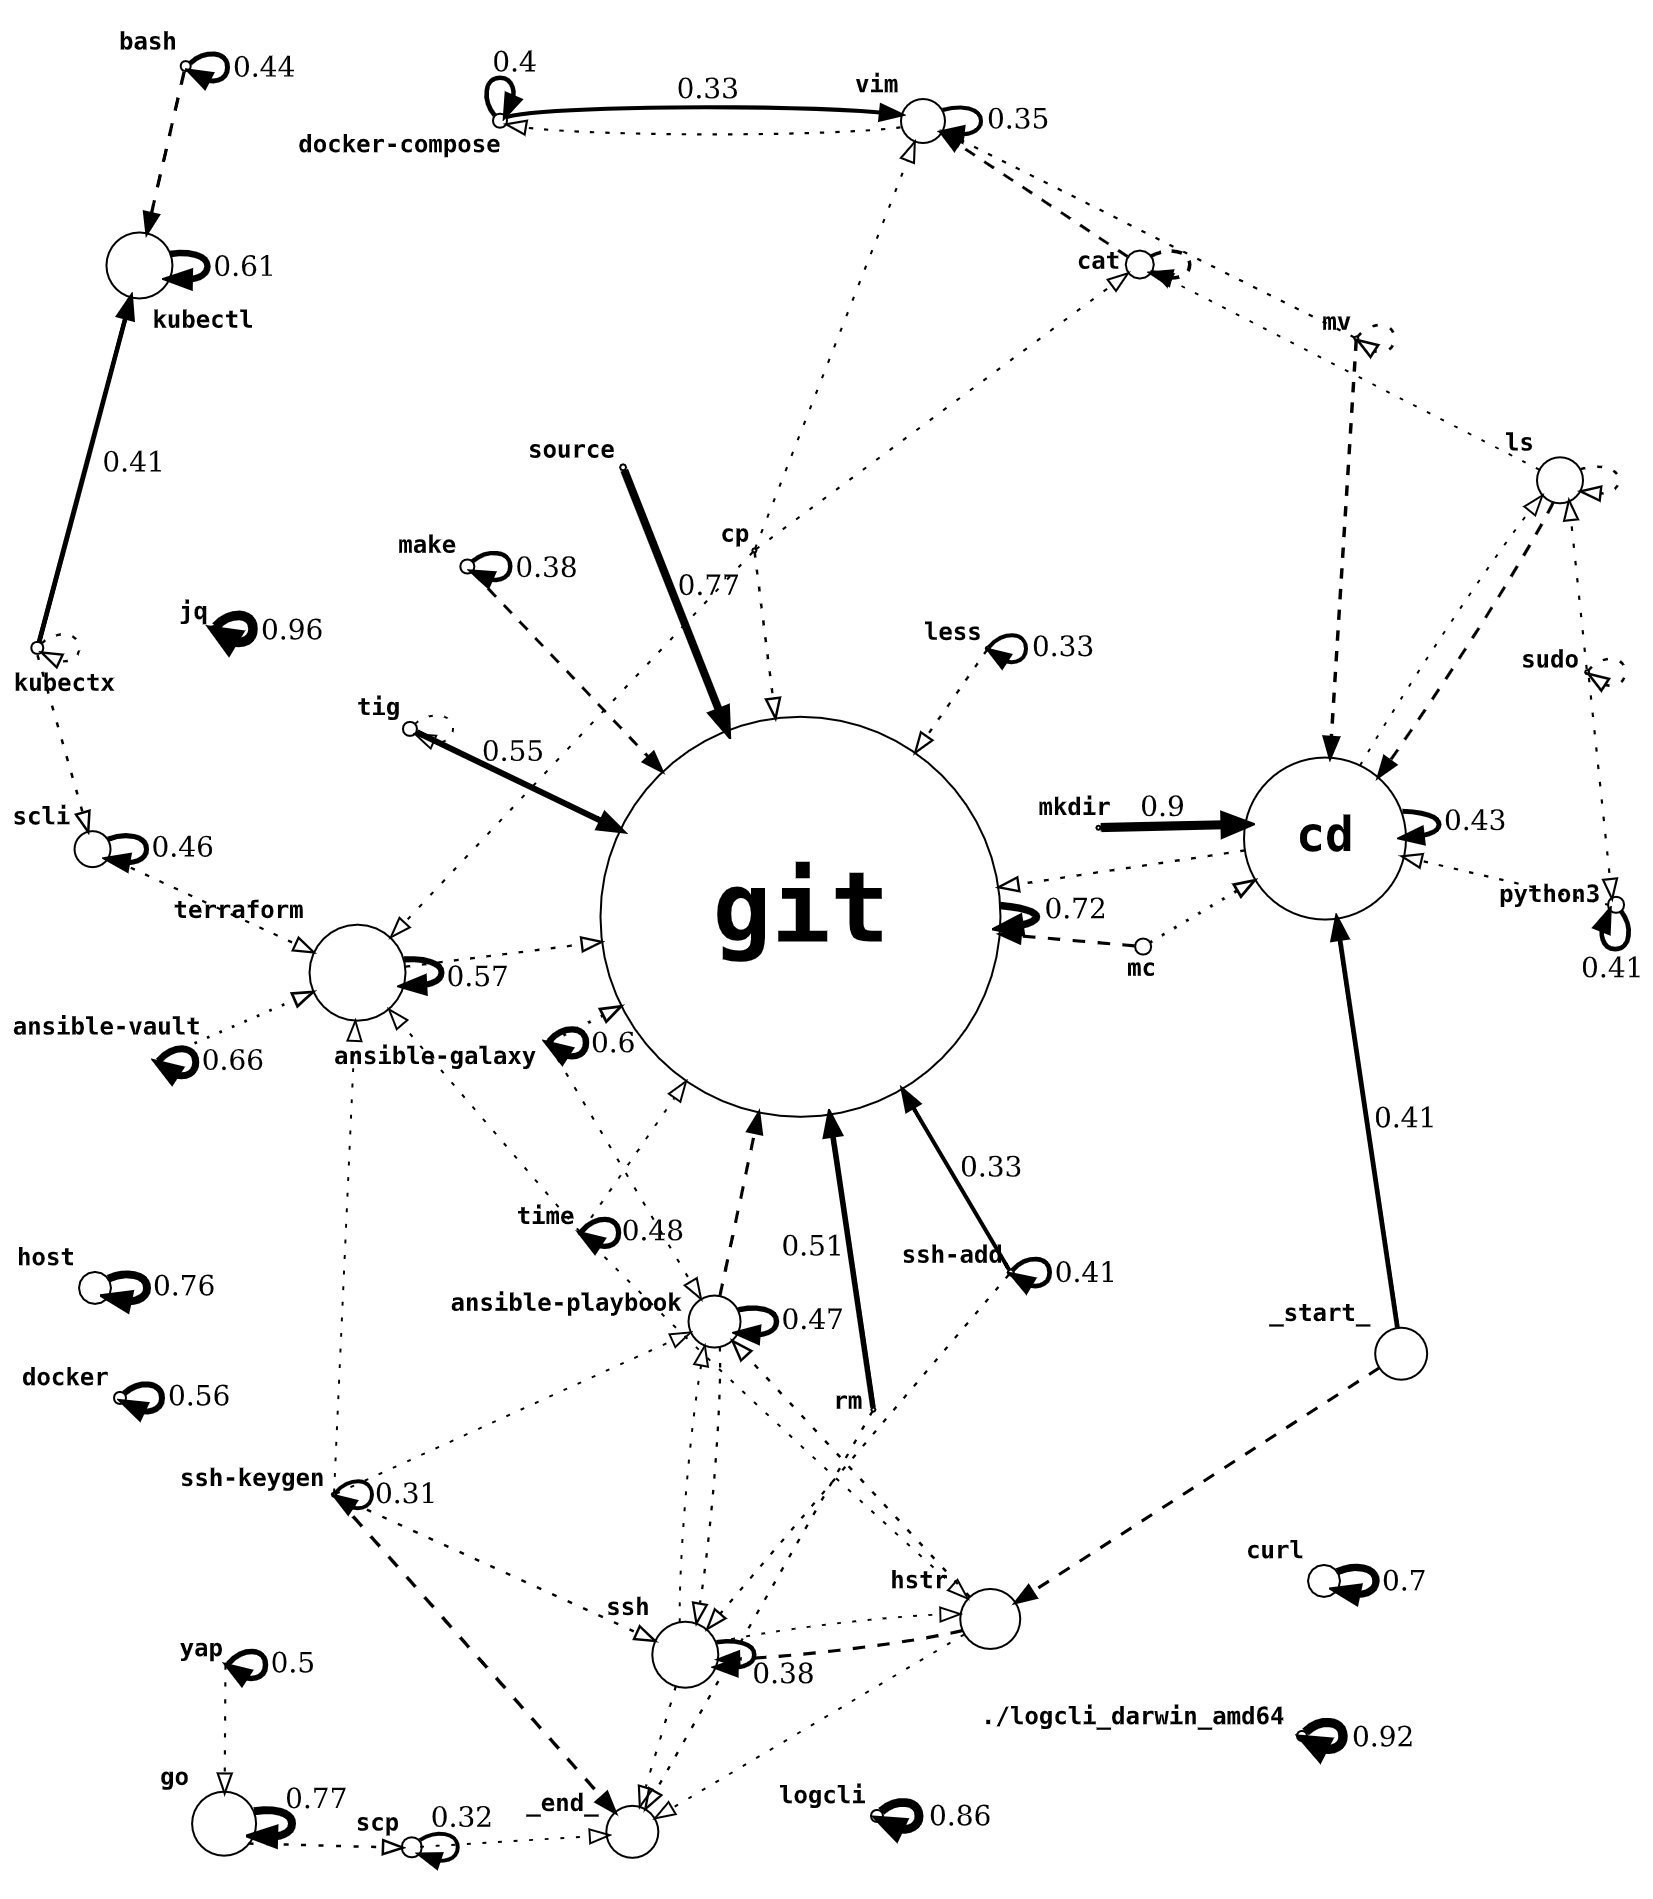
\includegraphics[width=\linewidth]{figures/greenberg_new/graph_cmd-sequence_vit_41_0-1_crop.png}}
  \caption{Sequential structure of command usage.}
  \label{seq-graph}
\end{figure}

\begin{figure}

\centering
\begin{tabular}{|l|l|}
\hline
Edge style & Transition probability            \\\hline
Regular/full     & 1.0 -- 0.3 (specified by labels) \\
Dashed      & 0.3 -- 0.2                         \\
Dotted      & 0.2 -- 0.1                         \\
\hline
\end{tabular}
\caption{Sequential structure of command usage (legend).}
\label{tab:seq-table}
\end{figure}

\todo{sequential graph and its legend table must be on the same page!}




% REF: "Through a multivariate analysis of UNIX commands invoked by the site population, Hanson, Kraut, and Farber (1984) examined the interaction effects between commands. Their results show statistically significant relationships between certain command chains; the relations between the fifty most frequently used commands are shown in Figure 3.3. Each ball in the network represents a command, its size indicates the usage frequency, and the arrow indicates the significant dependencies. One dimension of these relationships is modularity. Some commands, such as Is, are core commands - they are used frequently and are surrounded by many other commands (i.e., highly modular and independent). Others are not; they are surrounded by specific command sequences. An example of the latter is cp, which is generally preceded by itself and followed by chmod." "Commands are also related by functional clusters, such as editing, process management, orientation, social communication, and so on (Hanson, Kraut, and Farber, 1984), which may not be revealed by statistics."

\redtext{Greenberg concluded that assuming that the sequential dependencies of commands found by polling all the users together is a mistake.}

In earlier chapter, we saw that there are a big differences in vocabularies of different people so it is not surprising that sequential properties of the commands also differ significantly between individuals.

We created a graph sequential dependencies between commands for a selected individual. Since we are studying sequential properties of commands with the relation to history tools; We chose not to use the same method as Hanson so the graphs are not comparable. 

\todotext{TODO: polish this up}
We created the graph by taking 41 most used commands. Each node represents a command and the size of the node is proportionate to the command frequency. Each vertex represents a transition probability from one command to the next one. We decided to create the graph this way because it represents properties that could be potentially used in history tools; It only uses the probability of transition from one command to the next one. Hanson used a method which also considers the reverse transition probabilities; That is the probability that given command was preceded by the previous command. For example, when predicting the next command we only have the information about the past and current command. 


The \verb|_start_| command represents a start of a new terminal session.
The \verb|_end_| command represents an end of the terminal session; It does not matter how the session ended.

\todotext{Errors filtered out because we want to study the history to help people achieve their goals - filtering exit status !0 is not fully correct but the resulting data is more useful than without any filtering.}

\todotext{There are strong dependencies between certain commands - e.g. mkdir almost always followed cd - cd into the newly created directory, source is almost always followed by git w/o clear reason; Existence of strong dependencies suggests that it could be worth to predict the next command using the previous one.}

\todotext{Many commands have a high probability of being repeated - e.g. jq which is almost always followed by itself, curl, git, ssh ...; High rate of commands being repeated shows the need to recall recent history records - even the most immediate ones. Remember that these high rates of repeated commands are not caused only by errors and typos because all commands with non-zero status were filtered out.}

\todotext{Ad. above: Almost all commands repeat themselves with a significant probability. Some commands do not repeat themselves. E.g. hstr, rm, cp, source, mc ... these are simple commands that do not usually have many arguments and achieve simple goals that do not need to be repeated (remove file, copy file). It seems that commands with more arguments are repeated more A) because they help the user achieve complex goals B) the user adjusts the command because it is nontrivial to put it together the arguments C) command performs something fairly complex and user repeats the command (external change) }

\todotext{At the beginning of the session the user often changes to a different directory. Or they use hstr which is a history searching tool.}

\todotext{There are some very frequent commands that are used over and over again. This makes it easier to predict the next command. But it does not mean that it is easy to predict the next command line. Vast majority of these invocations only share the command but not the arguments.}

\todotext{Sequential graphs differ significantly between users. However, the findings described above could be also found in the sequential graphs of other users.}

\todo{highlight referenced nodes}

\todo{add words delete words}

\todo{NOTE: Summed up toolsmith \%\%\%}
 %The rank frequency distribution of command usage by groups of like and
%unlike users is approximated by a Zipf distribution.
%2. With a few exceptions, the frequency of use of most commands differs between
%groups - rank order is not maintained.
%3. There is little overlap between the command vocabulary of different users,
%even for those with apparently similar task requirements and expertise.
%4. Individuals have small command vocabularies, and new commands are acquired slowly and irregularly. Consequently, the Zipf model may not be an
%accurate estimate of an individual's behavior.
%5. Some commands cluster around or follow others in statistically significant
%ways, although these dependencies vary from one individual to another.



% \todotext{TODO: Greenberg conducted a study in his work \cite{greenberg1993computer} in 19XX which provides a lot of insight into how people use shell. It's not obvious that conclusions and ideas in the work still hold. To make sure that the usage of shell didn't change to the point where we can't use the ideas anymore. }


\subsection{Recurrence rate of command lines}

\redtext{In the previous sections we have examined how people use commands when interacting with a command line interface. Now we focus on whole command lines entered by the user. By \textit{command line entry}, we mean the line entered by the user as it appears in the shell history. Multi-line commands are considered a single command line entry.} 

\todotext{It is important to study command line entries because they contain the full information entered by the user. In contrast, commands only offer partial information. For example, even if we were able to predict the next command of the user with 100\% accuracy user would still have to type in all the arguments themselves. Usefulness of such history mechanism would not be great.}

\todotext{Greenberg has reported average recurrence rate of 73.8\% for all subjects; Recurrence rates for computer scientists and experienced programmers were 74.4\% and 67.7\% respectively. Average recurrence rate of command line entries in our data is 70.3\%. Based on descriptions of groups in \cite{greenberg1993computer} our subjects are computer scientists and experienced programmers.}

\todotext{High average recurrence rate shows the potential of shell history tools. The fact that command line entry was already entered by the user does not mean the user will recall it from history. For example, if remembering and retyping is easier than using history facilities there is no point in recalling the command line entry from the shell history. Naturally, longer command line entries are more likely to be recalled and shorter ones are more likely to be retyped. ... other factors of recall utility }

% Table 5.2. The average recurrence rate of the four sample UNIX user groups

\begin{table}[]
\centering
\begin{tabular}{lllll}
\hline \hline
Sample name             & \multicolumn{2}{c}{Recurrance rate} & \multicolumn{2}{c}{Range} \\
                        & mean             & std dev          & minimum     & maximum     \\ \hline
Novice Programers       & 80.4\%           & 7.2              & 64.7\%      & 91.7\%      \\
Experienced Programmers & 74.4\%           & 9.7              & 51.4\%      & 90\%        \\
Computer Scientists      & 67.7\%           & 8.2              & 46.4\%      & 82\%        \\
Non-programmers         & 69.4\%           & 8.1              & 50\%        & 84.3\%      \\
                        &                  &                  &             &             \\
Total                   & 73.8\%           & 9.6              & 46.4\%      & 91.7\%      \\ \hline \hline 
\end{tabular}
\caption{The average recurrence rate of the four sample UNIX user groups from \cite{greenberg1993computer}}
\label{tab:recurrence_rate}
\end{table}

% \begin{figure}
%   \tmpframe{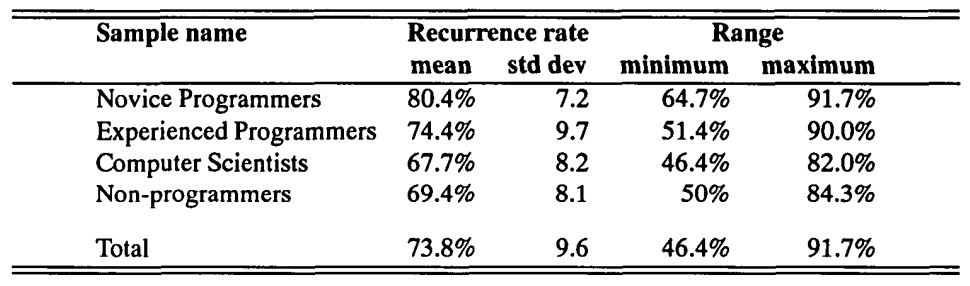
\includegraphics[width=\linewidth]{figures/greenberg/table_recurr-rate-in-different-samples.png}}
%   \caption{The average recurrence rate of the four sample UNIX user groups (Greenberg) \todotext{redo as an actual table}} 
% \end{figure}


\subsection{Maximum possible recalled characters}

\redtext{Recurrence rate represents how often people execute command line entries that were already entered before. Maximum possible recalled characters represents how many characters can be recalled from shell history assuming we store all previously entered commands. This metric show us the potential of shell history tools quantified in recalled characters.}

\todotext{TODO: Greenberg reports average command line entry length of 7.58 characters. Maximum possible recalled characters per command line submission was 4.43 characters. Whenever the user types in a new command line entry there can be no characters recalled; This lowers the maximum recalled characters per command line entry.}

\todotext{TODO: Our data shows average command line entry length of 29.26 characters. Maximum possible recalled characters per command line entry is 16.34 characters. We see a significant increase in the average command line entry compared to Greenberg. Naturally, this also increases the potential recalled characters.}

\redtext{This difference makes sense when we look at commands that are available today. There are new complex commands with subcommands and long options. Consider} \verb|git|\redtext{, it has many subcommands which accept different options; Additionally, the order of arguments matters.}

\todo{Is this where we talk about complex commands ??? }

\todotext{We conclude that the potential of shell history facilities has increased over the years because of differences in shell usage, available commands, and shell itself.}

\subsection{Maximum possible recalled characters including prefix matches}
% prefix matches

\todotext{TODO: We found situations in our collected shell history where the user gradually modified recently submitted command line entries. These entries often did not exactly match any of previous command lines entries but they were very similar. Workflows that repeat parts of previous command line entries are an opportunity for shell history use. Previously introduced metric does not account for this type of command line entry reuse. To estimate the potential of shell history tools we measured the potential recalled characters considering prefix matches.}

\todotext{TODO: Maximum possible recalled characters including prefix matches is 26.77 characters per command line entry. You can see that this is close to the average command line entry length; This means that almost all command line entries share prefixes of significant length with previously submitted command line entries. This of course does not mean that it is possible to create a shell history system that achieves these amounts of character reuse. However the potential of history facilities is great. }




\todo{NOTE: avg recurrence rate \& avg max possible recalled characters \%\%\%}
% ALL avg cmdline = 29.269552945461168
% >>> Avg recurrence rate = 70.29523637022278
% >>> Max avg recalled characters = 16.34658576344865
% >>> Max avg recalled characters (including prefix matches) = 26.770874841514217


% greenberg 1993 vs now
% the average length of command lines is 7.58
% recurrence rate is 74.4% for Experienced Programmers (avg group), max chars. recalled for an optimal conditioning method is 4.43 characters predicted per submission.

\blind

\subsection{Potential recalled characters as a function of distance}

\todotext{TODO: add graph with all subjects combined or separated}

\begin{figure}
\centering
  \tmpframe{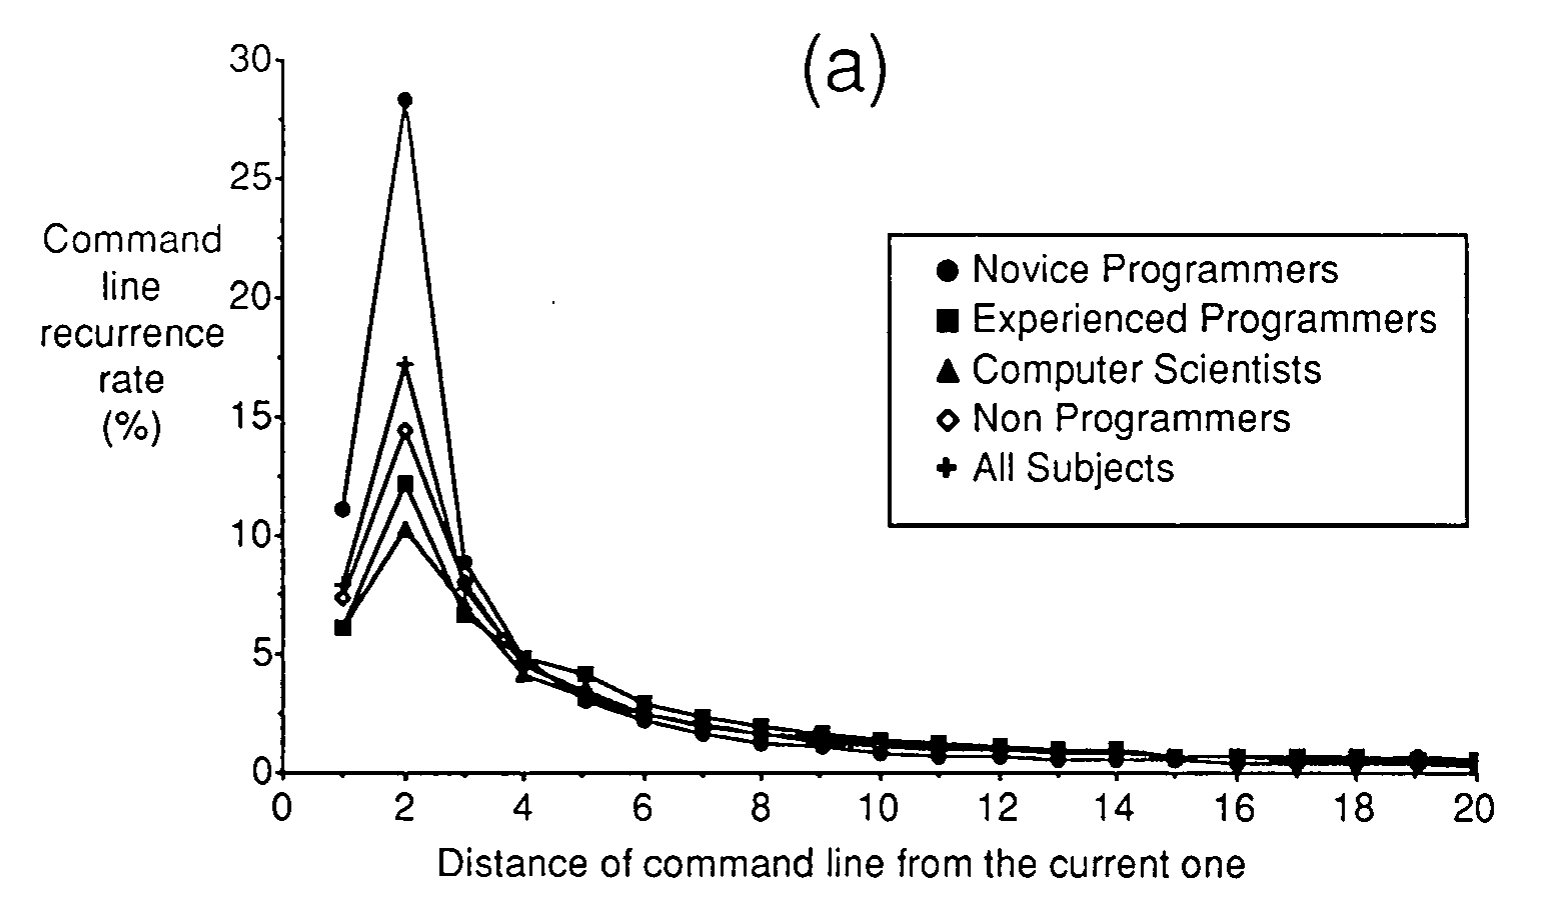
\includegraphics[width=\linewidth]{figures/greenberg/plot_ref_cmdline-recurr-rate.png}}
  \caption{Recurrence distribution as a measure of distance. (Greenberg)}
\end{figure}

\begin{figure}
\centering
  \tmpframe{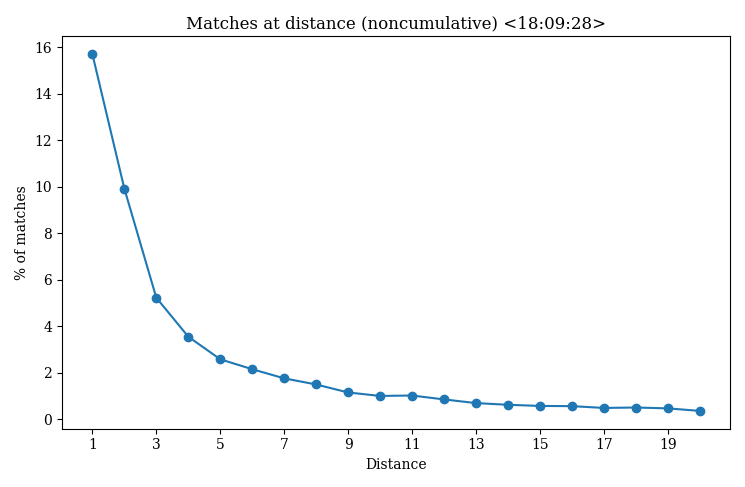
\includegraphics[width=\linewidth]{figures/greenberg_new/plot_cmdline-recurr-rate.png}} 
  \caption{Recurrence distribution as a measure of distance.}
\end{figure}


\subsection{Command line entry vocabulary}

\todotext{TODO: find out where to put this !!! }

\todo{!!! conclusions from plots !!!}



\todotext{}




% Figure 5.6. Command line vocabulary size vs. the number of commands entered for four typical individuals.

\begin{figure}
\centering
  \tmpframe{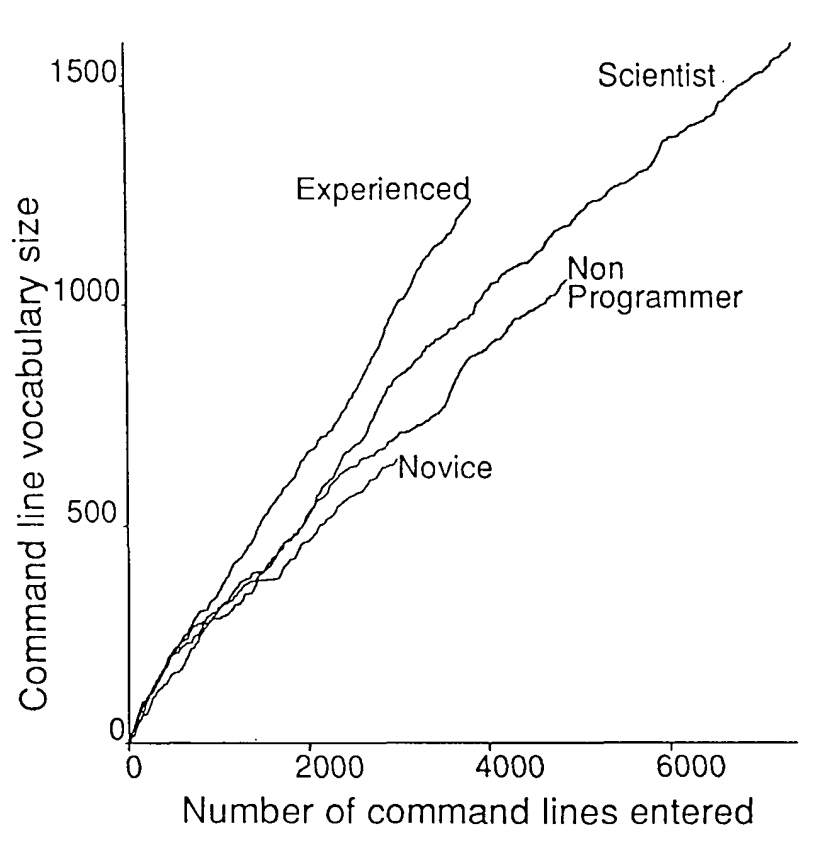
\includegraphics[width=0.6\linewidth]{figures/greenberg/plot_ref_cmdline-vocab-size.png}}
  \caption{Command line vocabulary size vs. the number of commands
entered for four typical individuals. (Greenberg)}
\end{figure}

\begin{figure}
  \tmpframe{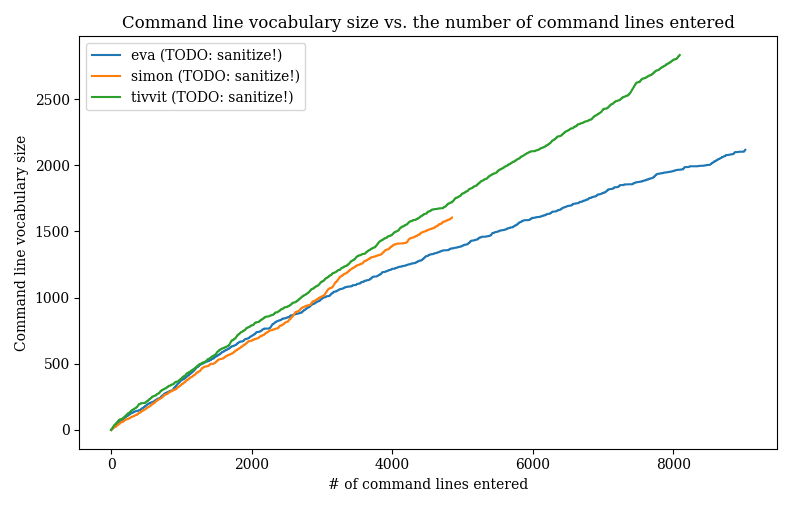
\includegraphics[width=\linewidth]{figures/greenberg_new/plot_cmdline-vocab-size.png}}
  \caption{Command line vocabulary size vs. the number of commands
entered for a single experienced programmer \todotext{TODO: title}}
\end{figure}

\subsection{Predicting command lines entered by users}
\todotext{TODO: Predicting users' next command line - what is the state of the art, what are the disadvantages}

\blind[2]


\todotext{How have shell usage changed since standard shell history features and greenberg study - longer commands, more commands; sessions (there can be more terminal windows open -> history is not strictly sequential anymore); }



\blind[3]


\section{How people use shell history}

\todo{DESC: practical chapter with concrete examples based on the standard history features}

In the previous sections, we have looked at existing research about shell usage. We compared the findings from literature with a small sample of data we collected ourselves. 

We saw that there is a lot of recurrence and patterns in the way people use shell. These properties of shell usage show us the potential of shell history. When designing any shell history tools we should leverage and respect them.

However, we should not blindly assume that leveraging the recurrence and patterns of shell usage will produce useful history tools. To see the full picture, we need to examine not only how people use shell but how they use shell history.  

For example, studying your shell usage could show us that you often use a specific command line entry. However, there is a significant difference in workflow based on whether you prefer to recall the entry from history or if you prefer to type it out. A shell history mechanism that suggests command line entries that you never retrieve from history provides zero value. 

Consider another example; You download and install a new history tool that is supposed to increase your productivity. It promises to predict what command line entry you are going to use next. It is activated when you press \verb|arrow_up|. There is an issue with such a tool; You are likely used to having access to recent history entries when you press \verb|arrow_up|. You probably have a strong expectation that \verb|arrow_up| gives you previous history entry; Chances are that sometimes you press \verb|arrow_up| and execute the retrieved history entry without even reading it. History tool that breaks this expectation will cause mistakes and ultimately you will be forced to either change your habits or uninstall the tool.  

\todo{TODO: Either use ARROW\_UP everywhere or arrow\_up}

\todotext{TODO: no usable research on how people use shell facilities (Greenberg has usage from csh with history expansion only)}
\todotext{TODO: to get an idea of how people use shell history we explored and "initiated/participated" in online discourse}
\blind 


\subsection{Online discourse about shell history}

\todotext{TODO: talk about our online research - my twitter thread, hackernews threads, SO questions, etc.}

\todotext{SO and SE show the standard issues, questions, wanted features}
\todotext{TW thread shown things people use and features they want}


\todotext{TODO: Naturally, people are selective about what they share online this skews the available information. People are not likely to share the basic usage habits they do not even realize they have. BUT they will share their custom configurations and scripts. }
% We find mentions of issues they run into when using standard history features.

\subsection{Common shell history issues and usage patterns}

\todotext{TODO: In this section, we present our observations and highlight sentiments that people voice online. Our observations include issues people face when using shell history, what people expect from shell history and ...}

\todotext{TODO: We focus on more general findings. We leave specific tools people use for a later section.}


\subsubsection*{Robustness/Reliability of standard shell history}

The most common issues people ask questions about are related to reliability of the history.
There are various reasons why certain command lines might not be saved to the shell history; This means that people experience situations, when they expect some entry to be present in the history  but they cannot find it because it is missing.

To understand why reliability is essential, imagine you are looking for a command line entry and you are absolutely certain you executed it in the past; In this situation, you could spend a significant amount of time trying to retrieve the command line entry from the history. You could give up at any time but how likely is that if you know that you executed the command line entry earlier.

The most common reason people lose portions of their shell history is caused by how shells handle multiple simultaneous shell sessions.    
\todotext{CONNECT}

People expect shell history to handle multiple simultaneous sessions gracefully. This is generally not the case; The user can run into multiple issues depending on what is the default configuration in the package provided by their distribution.

\todotext{The most common issue is - losing history from sessions because the last session overwrites the history file. Some people also expect the history to be shared between sessions which is nontrivial to set it up (in bash, zsh has an option)}


\todotext{The most severe issue is a race condition that can cause bash to lose the entire shell history. There is no mechanism that ensures that two shell sessions will not write out shell history at the same time. People have reported losing their whole history because of this issue. When users shutdown their machine with multiple open terminals the chance of the race condition increases because all the shell sessions will be "killed" by the "system" at roughly the same time.}

\todotext{Unlimited history - people expect it}
\todotext{unlimited search, some people experience their history being truncated on reboots}


\todotext{history as a Full transcript of actions - people expect}


\todotext{TODO: Shell history is not reliable enough -> People do not trust it -> They start using other solutions}
\todotext{Using other tools because of preference or convenience is okay. Using other tools because shell history does not feel reliable is a failure of shell history.}

\todotext{Many of these issues can be solved with a right configuration; However, this begs a question, should tools rely on additional configuration for the basic functionality to work properly?}


\subsubsection*{Basic/Standard shell history features/usage}
\todo{Not sure if this is the right place - it might be}
\todo{CONSIDER: This might get it's own subsection after all the common issues and feature requests/wishes}

\todotext{TODO: Recalling recent history}

\todotext{TODO: Simple stepping through history using arrow keys - failry straight-forward feature commonly used when people need to access recently executed command line entries.}

\todotext{TODO: Prefix search is realized by verb|history-search-backward| and verb|history-search-forward| readline functions in bash. It is very common to replace the simple stepping through history with prefix search; When you use prefix search with an empty line it works almost identically to stepping through history. Prefix search functionality is essentially a superset to stepping through history. }


\todotext{Prefix search is often praised in shells where it is enabled by default\footnote{The Fish shell and a popular configuration framework oh-my-zsh both come with a prefix search enabled by default and bound to verb|arrow\_up|} and it is often ignored in bash where one needs to configure it.}

\todotext{TODO: Reverse search}

\todotext{TODO: Reverse search is an interesting feature. Many people use it and find it useful. That makes sense because it is the most powerful interactive history mechanism available to users.} 

\todotext{There are a few issues with reverse search we should point out. Reverse search only shows one result at a time; To show the next one we can press verb|CTRL-R| repeatedly. Common issue people have is that when you press verb|CTRL-R| too many times it is not trivial to go back to the previous result.}

\todotext{TODO: Shows only one result - going through results one by one can be quite tiresome}

\todotext{The default keybinding for getting a previous result is verb|CTRL-S|. The issue is that verb|CTRL-S| is also commonly used for flow control. By default, in some distributions, pressing verb|CTRL-S| freezes all the input coming to the terminal. This can be quite obviously very confusing for new users. It is possible to configure verb|CTRL-S| to be free for forward history search; However, if people do not change the configuration they have no way to get to a previous search result.}

% Terminal can be unfrozen by pressing \verb|CTRL-Q|.

\todotext{TODO: Query in reverse search is consecutive - not ideal when we only remember parts of the command. E.g. ... ?}

\todotext{TODO: manual filtering}
\todotext{history | grep - gives you a lot of power and extensibility}
\todotext{This seems to be quite common.}
\todotext{Two takeaways: Interactive Std. history features may be lacking if people use manual filtering instead - lets try to fix it, AND people like extensible and standard solutions}


\todotext{TODO: History substitution}
\todotext{you don't see what you execute unless you enable the option - minority of people seem to use these (more than just individuals but not many people)}
\todotext{ !! is quite common, e.g. sudo !!}



\subsubsection*{Additional information in shell history}

A common sentiment we can find online is the wish to have additional information saved in shell history; The most frequently requested additional information is the current working directory and the time of the execution. Other requested information includes duration of the execution, user and host. 

Some people would also like if there was a way to filter out history entries with non-zero status or perhaps, even to not save them to history at all.

\redtext{We are going to cover the benefits and possibilities afforded by saving additional information to shell history in the later sections in detail.}

\subsubsection*{Control over what is saved to history}
Sometimes people do not want certain command line entries to be saved to history. 

It is very common to have the shell configured to not save duplicate entries to the history.  
Another common reason to not want a certain command line to be saved to history is when it contains some sensitive information. This is typically a password passed as an argument to an executable.

Other command line entries that some people do not want in their history are short useless commands and dangerous commands. An example of the former is \verb|ls| which is easier to type again than to recall from history; An example of the latter is \verb|rm -rf *| which could have catastrophic impact if recalled and executed by accident.

There are configuration options available that make it easy to filter what gets saved to history using simple pattern matching. There is also an option to ignore command line entries starting with a space; This is commonly used to prevent arbitrary commands from being saved to history.

It is worth noting that people sometimes want to delete history entries after they submitted them. Another workflow some people have is to disable saving of command line entries to history for the rest of the current session.

\subsubsection*{Shell history across multiple devices / Synchronizing history between devices}

\redtext{Quite a few people wish to have their shell history synchronized between multiple devices. This is not surprising because many services work independently of a device and the user data is often stored online. It is understandable that people expect their shell history to follow this trend.  }

\redtext{Some people shared workflows that involve reuse of shell history between devices. For example, someone wanted to have access to shell history from different machines when setting up new servers.}

\subsubsection*{Smart shell history features}

\todotext{TODO: A portion of questions we can find online is about features that would require the shell history to understand the contents of the submitted command line entries. This means that shell history would have to include at least a limited parsing of the shell. Examples of such features are expansion of aliases and transformation of relative paths to absolute ones. These expansions could make the history entries independent of set aliases and current working directory. }

\subsubsection*{ADDED: Full transcript}
\todotext{People sometimes with to have a full transcript of their actions - but history is deduplicated}

% Delete fron history

\subsection{Target users \redtext{MOVED (and typical workflows)} }

When designing any product, we need to make sure we know who the product is for. Shell history tools are no exception. To capture the target user-base we are modelling two typical users as personas. As the first persona we chose an experienced user because shell history tools are likely more for users that use shell extensively. As the second persona we chose a novice shell user; Designing tools for novice shell users can result in a product that is better for everyone. For example, it is especially important for novice users that the product is easy to install, comes with a good default configuration, and is easy to use for the first time; These characteristics are beneficial to everyone not just novice users. 

\todo{TODO!: User groups - find the common characteristics, describe the common characteristics}
\todotext{ understand shell options, do they speak english?, ... }

\todo{TODO!: personas should have concrete languages, editors they use, etc. }

\subsubsection*{Typical experienced shell user}

Experienced professional programmer \textit{Peter} develops, deploys, and operates back-end applications. Main languages he uses at work are C and C++. He has years of experience with developing on and for the Linux operating system. He is proficient in Bash and he written a few small shell scripts to increase his productivity.

His editor of choice is Vim; He has a sizable Vim configuration with multiple Vim plugins he collected over the years.

The shell he uses is Zsh with Oh-my-zsh \cite{toolsohmyzsh} shell configuration framework. On top of that he maintains a set of his own custom options and aliases. He puts the resulting configurations on his machines. He does not change his configuration often but he likes to be able to configure his shell and other tools he uses.

He often uses \verb|ssh| to log into remote machines; The remote machines are shared and have the default shell configuration. He keeps his shell and editor configuration somewhat similar to the default one because he does not want to constantly switch between very different environments. 

His daily shell workflows include complex commands with many long arguments. Switches between many different projects. When coming back to a project he sometimes cannot remember what command line entries he was using. He is familiar with Make but he often forgets to create Makefiles for typical tasks in projects.

He makes use of interactive history features like reverse search and prefix search. However, he quite often uses \verb#history | grep 'pattern1' | grep# \verb#'pattern2'# to manually filter shell history because it is both more powerful and sometimes feels easier to use than reverse search. Manual filtering allows him to search by more than one pattern and to see many of the matching results. 

\todotext{TODO: ADD challenges and benefits ? maybe}

\subsubsection*{Typical novice shell user}

Junior data analyst \textit{Mark} has recently started his first job. He uses shell because he needs it for his job. The primary language he uses is Python. 

The editor he uses is Visual Studio Code because it was recommended to him by a coworker. He likes that it suggests extensions to install based on files he is working with.

He is using Bash with the default configuration provided by Ubuntu distribution; Apart from that he does not have any custom shell configuration. 

Since he does not have much experience with shells, he neither does understand the shell configuration files nor he feels confident editing them. If he discovered or someone recommended a new shell tool to him he would prefer an installation without the need to edit the shell configuration files. Additionally, he expects any programs and tools he installs to work out-of-the-box and not to require much configuration. 

There are shell history features he is not aware of like history expansion and prefix search. He uses arrow keys to get recently submitted command line entries and he presses \verb|CTRL-R| when looking for history entries further in the past. 

\todotext{TODO: ADD challenges and benefits ? maybe}


\section{Common shell history workflows}

Now that we know who our target users are we can formulate common workflows for them. We do not specify the workflows for each of the target users separately; Instead, we comment on the difference between the users when necessary. \todo{we only ever make comments about the experience level of the users}

Workflows we formulate are based on previous research \cite{greenberg1993computer}, the online discourse we discussed earlier, discussions with potential users, and our own experience with shell history. Additionally, we collected and examined shell usage and history of a few users; This helped us to confirm and formulate the workflows.

\todotext{Workflows are simplified by using common commands to make them easy to understand. Some of them were shortened to fit onto the page. Real examples would contain commands specific to the individual users work and the command line submissions would be longer in some cases.}

\redtext{There is one more thing you should keep in mind when reading the examples; You, unlike the user, will have the full sequence of history entries in front of you. The user in the examples will often have only limited memory of the command line entries he submitted earlier. }



%\redtext{We grouped the workflows to several distinct categories; In each category we explain the  ...}
\redtext{In this section, we discuss how the users can complete these workflows using standard shell history features. We also point out the limits and shortcomings of the standard history mechanisms. }



\todo{TODO!: explicit sorting key for workflows - from the most recent to the less recent ones}

\todo{TODO!: consider bullet points to introduce the individual workflows}

\begin{itemize}
    \item Editing a preceding history entry
    \item Blindly recalling very recent history entries
    \item Retrieving recent history entries
    \item Editing recalled history entries
    \item Repeating a sequence of history entries
    \item Searching with limited knowledge
    \item Searching with implicit context
\end{itemize}

%Additional configurations and tools will be discussed in later sections.

\subsection{Editing a preceding history entry}

In this first workflow, the user submits a command line entry but is not satisfied with the result. To fix that, he retrieves the immediately preceding history entry, modifies it and executes it again. We will look at multiple example sequences of command line submissions for this workflow.

\begin{verbatim}
    wget https://pastebin.com/raw/EDELXNYp --silent
    wget https://pastebin.com/raw/EDELXNYp --quiet
\end{verbatim}
In this example, the user is trying to download a file from \verb|pastebin| using \verb|wget|. The first command ends with a non-zero exit status because \verb|--silent| is not an option of \verb|wget|. He presses \verb|ARROW_UP| to retrieve the previous command line entry, fixes the mistake and presses \verb|ENTER| to submit the command line entry again. 

Using \verb|ARROW_UP| is efficient in situations when we need to either edit the end of the command line entry or append to it. % Command line editing -> more efficiency
The next example shows a different case.

\begin{verbatim}
    apt-get install zsh
    sudo !!
\end{verbatim}

Here, the user wants to install the \verb|zsh| package. The command fails because superuser permissions are needed to install packages to the system. Instead of using interactive history features, the user uses csh-style history expansion \verb|!!| which repeats the previous history entry. 

By using \verb|!!| we can efficiently prepend or append to the previous command line entry. There are other csh-style history expansions but \verb|!!| is by far the most commonly used one. 

So far, we only saw situations where the submitted command line ended with a non-zero exit status and then the user fixed the error. This is not always the case because not all errors result in a non-zero exit code; Some errors are logical and not all programs respect the convention of properly signaling errors. Additionally, users sometimes gradually change and develop a command line entry to make sure that each step of the process works as intended. This is shown in the example below.

\begin{verbatim}
    sort data.txt
    sort data.txt | uniq -c
    sort data.txt | uniq -c > data_processed.txt
\end{verbatim}

In this next example, we see how the user processes \verb|data.txt| file. In each step, he uses \verb|ARROW_UP| to retrieve the previous history entry and continues editing it. When he is satisfied with the result, he redirects the processed data into a file. 

This example shows that there is not always an explicit error that could be detected by the shell to predict that the user will recall the previous history entry. It also shows that the editing process can be often continuous.

We just saw multiple different situations in which people continue working on the same command. We also saw different approaches to retrieving previous history entries. It is worth noting that in all of these situations the user relies on the sequential property of the history. 

% \subsubsection*{Retrieving recent history entries - \redtext{deprecated}}

% \todo{TODO: restructure - you can delete this intro, just give the surrounding text a quick read}
% In this second category, we consider workflows that involve retrieving \textit{recent} history entries. In this context, recent means that the user remembers the history entry they are looking for. \redtext{In all of these workflows the user also wants to retrieve the full history entry and execute it without any editing.}
% \todo{TODO: people do remember recent results vs. define recent as "people remember" }

% \todotext{MAIN: recalling recent and semi-recent commands "as exact matches", "recent" ~ the user remembers the command}

\subsection{Blindly recalling very recent history entries}

This second workflow is a retrieval and execution of a very recent history entry; The user remembers the exact position of the history entry he wants to recall. An example of such workflow is running the following sequence of command line submissions.
\begin{verbatim}
    make build
    vim hello_world.c
    make build
\end{verbatim}
First, we use \verb|make| to build a project. Then we edit a file using \verb|vim|. After that, we press \verb|ARROW_UP| twice and press \verb|ENTER| to execute the recalled history entry -- \verb|make build|. 

\todo{can be up to 3? arrow up's}
Consider, if we used a graphical editor or if we ran the editor from a different terminal; In such case, we would only have to press \verb|ARROW_UP| once but the workflow would essentially stay the same.

When recalling very recent commands the users often remember the exact position of the history entry; This means that they do not read the history entry that appears on the command line but they blindly execute it instead. This is an efficient workflow that shows us the importance of the order of recent history entries.

\subsection{Retrieving recent history entries}
The third workflow is a recall of history entry that is still recent but the user no longer remembers the exact position in the history list. This means that the user needs to read the history entries as they appear to see if the desired entry was retrieved. This is an example sequence of command line entries for this workflow.

\begin{verbatim}
    systemctl start nginx.service
    systemctl status nginx.service
    tail /var/log/nginx/error.log
    nginx -t
    vim /etc/nginx/nginx.conf
    nginx -t
    systemctl start nginx.service
\end{verbatim}

In this example, the user is trying to start an Nginx \cite{reese2008nginx} web server. At first, the server does not start and the command returns an error. The user quickly realizes that there is an syntactic error in the configuration file after checking it using \verb|nginx -t|. Then, the configuration is fixed using \verb|vim| and the syntax is checked again using \verb|nginx -t|. 

At this point, the user presses \verb|ARROW_UP| five or six times\footnote{This depends of whether or not they have history deduplication turned on.} to retrieve a recently executed command line entry \verb|systemctl start nginx.service|. Every time they press \verb|ARROW_UP| a single result appears and they need to read it. There is no way to tell if the desired result is one press of a button away, three, or seven. % When the user presses \verb|ARROW_UP| too many times they can show previous history entries by pressing \verb|ARROW_DOWN|.


% It seems that people experience the sunk cost fallacy\footnote{\redtext{TODO: describe?}} which combined with the lack of feedback from the system drives them to stick to the original plan -- pressing \verb|ARROW_UP|. 

You might think that people would not press \verb|ARROW_UP| five or six times and would rather use other history mechanisms.
The usage data we collected shows that even somebody who claimed to not press \verb|ARROW_UP| excessively actually does so quite often. Pressing \verb|ARROW_UP| five times is more common than you would expect and pressing it over ten times is rare but it still happens. We also quite often saw people pressing \verb|ARROW_UP| too many times and then using \verb|ARROW_DOWN| to go back to previous history entries; We think that it is easy to overshoot when you only see one history entry at a time.

\todo{we could include reasons why people do this but I don't think it's necessary/important (see drafts in comments)}

% 1-2 was the most common ... 5-6 quite common ... 8 - 10 rare  20 exceptions
% WHY: sunk cost fallacy + lack of feedback from the system
% WHY: people might not realize how far the entry is in the first place
% WHY: people do not want to "abandon the effort they have already put in" because anytime the result could be there

%It seems that in situations like this one people do remember the history entry well and perceive it as recent. This is why they chose to use  

\paragraph{History prefix search \redtext{TODO: next title, same workflow}}

An efficient alternative way to fulfil the same workflow is to use history prefix search. To use prefix search the user needs to remember the first word or at least the first few characters of the command line entry; This is very likely since all the command line entries we are retrieving in this workflow are recent.

We will use the example with Nginx to compare using prefix search with just pressing \verb|ARROW_UP|. When using prefix search, the user types in a prefix -- \verb|systemctl| -- and presses \verb|ARROW_UP| twice to get to the desired history entry. In contrast, when only using \verb|ARROW_UP| it took five or six presses to get to the history entry.

This might not seem like an improvement because we need to type the prefix before we start pressing \verb|ARROW_UP|. However, we have to realize that going through multiple history entries and reading them one by one requires a significant amount of time and effort compared to typing. 
    
This is a good example of how the number of keystrokes is not the only thing we should be taking into account; Generally speaking, shell history should save effort and time of its users. This means both the physical typing and the cognitive overhead required to retrieve the entries.
% REF(greenberg): Recurring inputs should be reentered more easily than the user's original entry, with the aim of reducing both physical tedium and the cognitive overhead of remembering past inputs. Reuse facilities should not be targeted only to experts, as they can help everyone.

% the prefix could be shorter e.g. "sys", "system"  ... typing vs. effort required to decide how long/short prefix is sufficient

\todotext{Is this ending good? - continue (check comments)}

% ADD(polished?): There is a vocal group of people with strong preference for prefix search. The rest of the people either do not know that prefix search exists, do not have it configured, or prefer plain \verb|ARROW_UP| possibly out of habit.
% NOTE: maybe this^ belongs earlier? (but maybe not)


\subsection{Editing recalled history entries}

In the precious section, we saw a workflow where the user retrieved a recent history entry and executed it again as is. Now, we are going to look at a similar workflow where the user retrieves a history entry, edits it and then executes it again. Workflows with editing are a little less common than the ones with direct execution according to the usage data we collected. An example of a workflow with editing follows.

\begin{verbatim}
    curl --data "value=test" http://localhost:8080/submit
    git add pkg/submit/submit.go
    git commit --message "fix submit endpoint"
    git tag v2.4.0-rc.1
    git push
    git push --tags
    curl --data "value=test" http://test.example.com:8080/submit
\end{verbatim}


Here, the user is using \verb|curl| to test a server endpoint running locally at \verb|localhost:3000/submit|. \todo{Check overflow} After being done with the testing they commit the changes, tag the version as a pre-release\footnote{Here "rc" in "v2.4.0-rc.1" version stands for release candidate which is sometimes used to mark pre-release versions.}, and pushes both commits and tags to the upstream. This triggers a CI pipeline that deploys the new version to testing environment. The user wants to test that the endpoint also works there.

At this point, the user presses \verb|ARROW_UP| six times to get to the desired history entry. Alternatively, he could use prefix search which would be more efficient.

After retrieving the desired history entry, the user needs to edit it to change the server URL from \verb|localhost| to \verb|test.example.com|. He holds down \verb|ARROW_LEFT| for a about a second, holds down \verb|DELETE| for about a second, types \verb|test.example.com|, and finally executes the changed command line entry. 

This seems a little tedious but it is still more efficient than typing the whole command line entry from scratch. Instead of navigating by and deleting single characters, we could use \verb|CTRL+ARROW_LEFT| to navigate by words and \verb|ALT+BACKSPACE| to delete whole words; This would be faster and more efficient. However, it seems that many people do not use the command line editing functions.\todo{TODO: Ask more people, so far more people use it than I expected}

This workflow shows us how people edit history entries after they retrieve them. We see that standard history mechanisms make it possible to edit history entries after retrieval. Reverse search, which we did not see in any workflow yet, is not an exception. This is a useful property that we should include in our designs as well. 

\todo{Is this the right order?}
\subsection{Repeating a sequence of history entries}\label{workflow-repeating-a-sequence}

In this workflow, the user has executed a sequence of command line entries and wants to retrieve and repeat all the command line entries in the sequence. 
Consider a following example.

\begin{verbatim}
    gcc generate_dot.c -o generate_dot.out
    ./generate_dot.out > graph.dot
    dot -Tpng -ograph.png graph.dot
    feh graph.png
    gcc generate_dot.c -o generate_dot.out
    ./generate_dot.out > graph.dot
    dot -Tpng -ograph.png graph.dot
    feh graph.png
\end{verbatim}
\todo{Consider removing the second repetition}
\todo{Actually test these commands (I wrote this using my memory and help pages)}

In this example, we are editing the \verb|generate_dot.c| file in another window. In this terminal, we compile a source file \verb|generate_dot.c|, generate a graph in the DOT\cite{graphvizthedotlanguage} language, run Graphviz\cite{ellson2001graphviz} command \verb|dot| to generate an image, and finally use image viewer \verb|feh|\cite{toolsfeh} to display the image.

% ALT (too long): After observing the resulting image, we edit the source file \verb|generate_dot.c| in another window.
After observing the image, we edit the source file \verb|generate_dot.c| in another window.
Now, we want to repeat the whole process of generating the graph and view the resulting image. To retrieve the \verb|gcc| history entry, we press \verb|ARROW_UP| four times. Retrieving the next \verb|./generate_dot.out| entry also takes four presses of \verb|ARROW_UP|. Similarly, we need four key presses for each of \verb|dot| and \verb|feh| history entries. 

We need four key presses every time because with each executed command line entry we are pushing all the history entries further back in the history. We see that using \verb|ARROW_UP| to repeat a block of history entries is quite inefficient.  

There is other standard history mechanism we could use to repeat a block of history entries; 
Executing \verb|fc -4 -1| opens an editor with last four history entries and then, closing the editor executes the commands. This, however, is quite cumbersome in practice and not many people seem to use it. 

%Alternatively, we could use history expansion \verb|!-4| to recall and execute the fourth previous history entry; However, history expansion is not saved to 
\todo{Consider mentioning history expansion (see comment)}
%\verb|!-4| works in a similar way

Repeating a sequence of history entries is not the most common workflow. However, it shows us the limits and inefficiencies of standard shell history.


\subsection{Searching with limited knowledge}\label{workflow-search-w-limited-knowledge}

In all the workflows we discussed so far, the user wanted to recall a fairly recent history entry. Now, we move on to workflows where the user searches for history entries that are older. In these workflows, the memory of the user is often a limiting factor; Both the knowledge of shell history and the desired command line entry is limited.

Below, we see an example for such workflow; The upper part are relevant history entries and at the bottom we see the command line entry the user wants to find. 

%This means that simply pressing \verb|ARROW_UP| is no longer an effective way to retrieve them.
% \redtext{We are going to look at multiple examples of workflow where the user searches for an older. We will discuss how the workflow changes when the user remembers less and less information about the desired history entry. The first example follows.}

%    curl -o /dev/null http://speedtest.tele2.net/100MB.zip

%    curl https://api.github.com/repos/curusarn/resh/releases \
%        --silent | jq '.[0] | .tag_name' -r
        
% curl --data "value=test" http://localhost:8080/submit

\begin{verbatim}
# relevant history entries:
    cd git/thumbnail_api
    ssh root@thumbnail-api.dev.example.com
    scp root@thumbnail-api.dev.example.com:/log/thumbnail/1.log
    git commit -m "improve api logging"
    ...
    cd git/thumbnail_worker
    ssh root@thumbnail-worker-1.dev.example.com
    ssh root@thumbnail-worker-2.dev.example.com
    ssh root@thumbnail-worker-3.dev.example.com
    ...
    ssh 192.168.2.105
# desired command line entry:
    ssh root@thumbnail-api.dev.example.com
\end{verbatim}

In the example above, the user wants to remotely login to a \verb|thumbnail api| server in development environment using \verb|ssh|. 

If the user saw the full example in front of him as we do now it would be quite easy to choose a good searching strategy. However, the user does not see nor he remembers all the relevant information. He will need to make use of his limited memory to find the desired command line entry. 

A common way to search shell history is reverse search; The user initiates reverse search by pressing \verb|CTRL+R| and types in the query \verb|thumbnail|. Resulting prompt is shown below.\footnote{The search result and the prompt should be on the same line; We moved them to separate lines because they would not fit the page otherwise.}
% Reverse search displays a single most recent history entry that matches the query  

\begin{verbatim}
(reverse-i-search)`thumbnail': 
    ssh root@thumbnail-worker-3.dev.example.com
\end{verbatim}

Here, we see that the \verb|thumbnail| query matched a history entry that is not very relevant. The user makes the query more specific by typing \verb|-api|.

\begin{verbatim}
(reverse-i-search)`thumbnail-api': 
    scp root@thumbnail-api.dev.example.com:/log/thumbnail/1.log
\end{verbatim}

The reverse search still does not show the desired history entry but it shows an entry that is much closer to what the user is looking for. The user thinks that the query is specific enough and presses \verb|CTRL+R| to show the next search result.

\begin{verbatim}
(reverse-i-search)`thumbnail-api':
    ssh root@thumbnail-api.dev.example.com
\end{verbatim}

The next result is the desired history entry. This was a pretty efficient but also a quite idealistic reverse search example. It worked out so well because the user was able to provide a specific enough query -- \verb|thumbnail-api|. We should look at a more realistic situation where the user struggles to come up with such query. %We will use the same shell history and desired command line entry as in the previous case. (same sentence as the start of the ne)
\paragraph{\redtext{TODO: title} Limits of history reverse search}

In this example, we are using the same shell history and desired command line entry as in the previous example. Again, the user wants to remotely login to a \verb|thumbnail api| server in development environment using \verb|ssh|. He presses \verb|CTRL+R| and starts searching using \verb|ssh| as a query; It is actually very natural and quite common to use the beginning of the line as a query in reverse search.

\begin{verbatim}
(reverse-i-search)`ssh': ssh 192.168.2.105
\end{verbatim}

The most recent matched history entry does not look very promising. The user tries to extend the query to \verb|ssh thumbnail|.

\begin{verbatim}
(failed reverse-i-search)`ssh thumbnail': ssh 192.168.2.105
\end{verbatim}

Here, we see how the user struggles to make the query more specific; Extending the query requires knowledge of the details of the desired command line entry. The user does not remember that he should be logging in under \verb|root|.  % It is exactly details like this one that we hope to retrieve from shell history so that we do not need to remember them. 

The user sees that the search has failed and so he aborts it by pressing \verb|CTRL+C|. He starts over by pressing \verb|CTRL+R|, typing \verb|thumbnail|, and hoping for better results.

% Shell history should be helping people to reconstruct history entries from pieces. Should people remember details about the history entries in order to be able to retrieve them?

% It is worth noting that there could be explicit \verb|failed reverse-i-search| is preferable to ...
% there could be other unrelated history entries matching the query; This false promise would likely lead to more time wasted searching.

\begin{verbatim}
(reverse-i-search)`thumbnail':
    ssh root@thumbnail-worker-3.dev.example.com
\end{verbatim}

This result is an improvement over the previous one. However, it is still far from what we are looking for. The user should extend the query to make it more specific. 

Previously, we assumed that the user remembers enough to extend the query to \verb|thumbnail-api|; That is a bold assumption. What if the user does not remember that words \verb|thumbnail| and \verb|api| are adjacent or that they are delimited by a dash symbol? In practice, it is hard to come up with a query that only matches the desired history entry; Oftentimes the query matches many other history entries which forces us to go through multiple search results.


The user is in a similar situation. He presses \verb|CTRL+R| repeatedly to display the search results one by one. At first, the user presses \verb|CTRL+R| slowly to have enough time to read the results. After about three key presses he becomes impatient and speeds up. This does not leave enough time to properly read each of the results which causes him to press \verb|CTRL+R| one too many times.

\begin{verbatim}
(reverse-i-search)`thumbnail': cd git/thumbnail_api
\end{verbatim}

The user knows that pressing \verb|CTRL+S| \textit{should} bring back the previous result. However, he also knows that pressing \verb|CTRL+S| freezes all input coming to his terminal; This is the default\footnote{Default configuration on many popular distributions has CTRL+S bound to generate XOFF -- the software flow control sequence that stops all input coming to the terminal.} behaviour and he could never be bothered to find out how to fix it.

At this point, the user gets annoyed because the only option is to start over. He aborts the search, presses \verb|CTRL+R|, and types in the query \verb|thumbnail|. Then, it takes five presses of \verb|CTRL+R| to get to the desired result; This time he is more careful to not go too far again.


\paragraph{\redtext{TODO: title: why reverse search sucks}}

As we just saw, the reverse search is not always an effective way to search the shell history. It heavily relies on the ability of the user to form a single continuous query; A single query that is specific enough to match the desired history entry without matching many other history entries. 

This drawback is further amplified by the reverse search only displaying a single result at a time. Displaying multiple results at a time would make it easier to find the desired history entry in cases when there are many matching results. 

Despite these downsides, the reverse search is a quite popular way to search the shell history. Why do people use it given the disadvantages we discussed? The reverse search is not without its flaws but it is still the most powerful interactive way to search the shell history. 

If the reverse search is as bad as we claim are there other alternatives that people choose to use instead? Another very popular method people use is manual history filtering. Manual filtering searches the history non-interactively; It brings its own set of advantages and disadvantages which we cover in the next section.


%There are two fundamental issues with it. 
\todo{MOVE this vvv  a bit later (SEE comments)}
% The first issue is that reverse search only accepts a single query. This limits the expressiveness of the search and disrupts the workflow of the user. 
% ***This is just not very useful if you remember multiple different parts of the command line entry.
% Ad. expressiveness: ssh, thumbnail, and api are all good queries, the user is certain that they match the desired history entry but they are not specific enough individually. Put them together and they match the desired history entry and nothing else.
% Ad. workflow: Once the user types in ssh as a query and finds out it is not specific enough, they are forced to throw it away and try a different one. Continuously adding more information = single workflow. Being forced to delete already entered information = breaking the workflow.

% The second issue is that it only shows one result. This amplifies the the first issue because if you could see multiple results easily you would not need such a specific query anymore. Having more results displayed at once would allow the user to skim the page. 

% to design, we can argue that single-result approach works great on arrow_up for quick access 
%            then we start to see some disadvantages when people use arrow_up to recall not-so-recent entries
%            finally the single-result (+single-query) approach completely breaks down when used in reverse search

% EDGE: Reverse search is one of a very few available ways to search shell history which unfortunately makes it very common. 
% EDGE: When we analyze reverse search we find out that it is a peculiar combination of features that bring the worst out of one another.


% EXTRA ISSUE: once reverse search fails you there is no way back


\paragraph{\redtext{TODO title}Manual history filtering}

As mentioned before, manual filtering is a popular non-interactive way to search the shell history. It can be used to fulfil similar workflows as the reverse search. To properly compare the two methods we will use the same example as before; You can see the same relevant history entries with the same desired history entry below.


\begin{verbatim}
# relevant history entries:
    cd git/thumbnail_api
    ssh root@thumbnail-api.dev.example.com
    scp root@thumbnail-api.dev.example.com:/log/thumbnail/1.log
    git commit -m "improve api logging"
    ...
    cd git/thumbnail_worker
    ssh root@thumbnail-worker-1.dev.example.com
    ssh root@thumbnail-worker-2.dev.example.com
    ssh root@thumbnail-worker-3.dev.example.com
    ...
    ssh 192.168.2.105
# desired command line entry:
    ssh root@thumbnail-api.dev.example.com
\end{verbatim}

As in the previous examples, the user wants to remotely login to the \verb|thumbnail| \verb|api| server in development environment using \verb|ssh|. He uses the \verb|history| built-in to print the shell history together with the \verb|grep| command to filter the history entries.

First, he types \verb#history | grep ssh#; The output could look something like this.

\begin{verbatim}
$ history | grep ssh
...    ...
421    ssh root@thumbnail-api.dev.example.com
450    ssh root@thumbnail-worker-1.dev.example.com
451    ssh root@thumbnail-worker-2.dev.example.com
452    ssh root@thumbnail-worker-3.dev.example.com
489    ssh 192.168.2.105
\end{verbatim}


Using manual filtering displays all five matching history entries at the same time. The user can skim trough the results looking for the desired history entry. 
After he finds the result, he can either copy and paste it using a mouse or he can use history expansion.

The user found the desired history in the list and uses history expansion to execute it; He types \verb|!421| and presses \verb|ENTER|.

\begin{verbatim}
$ !421
    ssh root@thumbnail-api.dev.example.com
\end{verbatim}

This was pretty quick and efficient. However, what if there were more matching history entries? What if the user could not spot the desired history entry in the list of results?

In such case, nothing prevents the user from further filtering the results. Pressing  \verb|ARROW_UP| retrieves the previous command line entry and typing \verb#| grep thumbnail# adds another query. He can repeat this until he is happy with the filtered results.

\begin{verbatim}
$ history | grep ssh | grep thumbnail | grep api
421    ssh root@thumbnail-api.dev.example.com
\end{verbatim}

Here, the combination of queries filtered out all history entries but the desired one.

We see that manual filtering has some clear advantages over reverse search.
First, skimming through the displayed results is relatively quick. This allows us to use queries that are not very specific.
Even generic query like \verb|ssh| that was not specific enough for reverse search gave us some useful results when filtering manually.

Additionally, in situation when the query is not specific enough, it is easy to combine multiple queries together. This makes manual filtering much more powerful than the reverse search. 
When using the reverse search we had to choose between the queries. Here we can use all of them; This results in a very flexible workflow where we refine the search instead of guessing which single query we should use.


As we already mentioned earlier, manual filtering is a non-interactive history mechanism. This comes with an obvious disadvantage; To filter history manually the user has to type extra characters \verb#history | grep# instead of simply pressing \verb|CTRL+R| to initiate the reverse search. In some situations, the reverse search might be a more effective way to search the history.

It is important to realize that manual history filtering is essentially just a use of standard shell utilities for searching history.
This makes it more appealing to experienced shell users because they use what they already know. At the same time, novice users who are not familiar with \verb|grep| and shell pipes may have a hard time even understanding how manual filtering works. 

\todo{If this feels like there is a conclusion missing check the comments vvv}

% the most powerful option to search is not easily available to novice users - this is understandable but not ideal (we should not assume that people who don't know shell basics do not need powerful history search)
% +++ we saw other examples of workflows with history mechanisms that not everyone knows of, but this the first one where it is the only options because the alternatives are not just less efficient - they won't find the result at all (in a significant number of situations)

% NOTE: Seems like a lot of effort BUT recreating the command line entry from scratch would take even more effort.

% SUMMARY: By using the shell history in this workflow, the user not only saved himself some typing but also remembering of the command line entries. Recreating old history entries from scratch often takes a lot of effort because it is not just a matter of typing. The saved effort by history during this workflow is significant. This also means that people are generally willing to spend more effort searching for the desired history entry because of the effort they would have to "spend" otherwise.


\subsection{Searching with implicit context \redtext{TODO: better title}}\label{workflow-search-w-implicit-context}
% GOOD vvv
In the previous workflows we saw that searching history heavily relies on the memory of the user. When the user does not remember enough the efficiency of the standard history searching mechanisms is reduced.

Now, we consider situations where it is possible to at least partially replace the knowledge of the user by other information; In following examples, we will see how we could improve the shell history by using additional information such as exit status or current working directory.

% dd if=~/Downloads/manjaro-kde-19.0-200224-linux54.iso \
%       of=/dev/sdc bs=4M status=progress oflag=sync
% sudo dd if=~/Downloads/manjaro-kde-19.0-200224-linux54.iso \
%       of=/dev/sdc bs=4M status=progress oflag=sync
    
% # <dozens or hundreds of command line entries>
    
% sudo dd if=~/Downloads/manjaro-kde-19.0-200224-linux54.iso \
%        of=/dev/sdc bs=4M status=progress
\begin{verbatim}
# relevant history entries:        
    dd if=~/ubuntu.iso of=/dev/sdc bs=4M status=progress
    sudo dd if=~/ubuntu.iso of=/dev/sdc bs=4M status=progress
    dd if=~/manjaro.iso of=/dev/sdc bs=4M status=progress
    sudo dd if=~/manjaro.iso of=/dev/sdc bs=4M status=progress
\end{verbatim}

In this example, the user wants to use \verb|dd| to create a bootable USB drive from an iso file. The user uses \verb|dd| as a search query. We are not considering a specific existing history mechanism. Instead, we discuss possibilities and potential of shell history in this specific situation.

All of the history entries in the example match the query. However, not all of these history entries are actually useful; Two of the entries that do not start with \verb|sudo| will result in an error if executed\footnote{We assume that the user is not currently logged in as a superuser.}. 

In situations like this one, it could be useful if the history entries that originally ended with a zero status code were displayed before the ones that failed. Reordering search results could help the user to find the relevant results more quickly. 

% +++ In this example it is directly visible that sudo is missing
% However, in other cases the difference could be more subtle like a misspelled option
% 
% Even in this example, this might not be immediately apparent. 
%
% Reordering is a better strategy then completely filtering out the results. The user can still pick any history entry he wants because none of them are missing.
%
%Reordering is non-invasive - not all entries with non-zero status are worthless so we want to keep them


\paragraph{\redtext{TODO: title} Directory sensitive history}


%# history from ~/git/image_server directory:

\begin{verbatim}
# relevant history entries:
    cd ~/git/image_server
    git pull
    vim pkg/encoder/encoder.go pkg/encoder/util.go
    make build
    make build && ./scripts/run_tests.sh --quick
    git commit -am "refactor encoding"
    ssh root@image-server-2.c137.dev.example.com
    ssh root@processing-node-13.c137.dev.example.com
    VERSION=2.4.2 make release
    git commit -am "release 2.4.2"
    git tag v2.4.2
    git push
    git push --tags
\end{verbatim}

Here, we see a section of shell history related to a specific project. The user executed all of the command line entries above a long time ago in the \verb|~/git/image_server/| directory. He did not work on the \verb|image_server| project since. This means that he does not remember these history entries and his history is filled with many other command line entries he executed since.

The user comes back to the project by typing and executing \verb|cd ~/git/| \verb|image_server|\todo{CHECK: verb overflow -$>$ verb split}. He wants to continue working on the project. He knows that he needs to edit some code, build the project, test it, and release a new version. However, he does not remember concrete command line entries for these tasks. 

Some of the command line entries he needs are easy to remember because they are generic; Examples of such entries are \verb|git pull| which pulls new changes from upstream and \verb|make build| which build the project. However, some of the tasks require knowledge specific to this project. For example, it might take some effort to find out that running tests is done using \verb|./script/run_tests.sh|. Similarly, it is not obvious that \verb|VERSION| environment variable should be set when running \verb|make release|.

This information is stored in the shell history but it is not easy to retrieve. Standard history mechanisms only search by the command line entry itself. It could be very useful if the user was able to display and search the history from the current directory.




%In situations like these, the user is essentially rediscovering the workflow for the project. This is very inefficient given that all the relevant history entries are already stored in the shell history. The issue is that retrieving the relevant entries using standard history mechanisms is very hard. The command line entry itself does not contain enough 

%with standard history is that none of the available history mechanisms allow us to retrieve the history entries we need. 


%It would be useful if the necessary information could be retrieved from somewhere instead of being rediscovered over and over again. 


% makefiles help

%Makefiles can help solve this issue; They contain command line entries needed to work with a specific project. However, not all command line entries are saved to Makefiles.

%people often use command line entries without saving them to the Makefile. 







%it would be useful if the user did not have to spend time rediscovering the workflow  could retrieve relevant history entries from history. 
% often it is hard/impossible to tell that the history belongs to the directory 
% many of the history entries 
% the server url is possibly useful but based on its name you would never say so

% there is useful info in history related to the project
% this info is in history but it cant be searched using standard history mechanisms


%We need to realize that many of these  history entries 
%Another example is the server URL \verb|processing-node-13.c137.dev.example.com|\todo{Overflow?} which is probably related to this project but .

%In situations like this one, the user could benefit from being able to access the shell history based on the current directory. 



\subsubsection*{History as a transcript}
%These are also less common but requested

\subsubsection*{Delete specific entry from history}

% see the full process how something was done, w/o deduplication
\todotext{USECASE: Retrieve a transcript of command line usage around certain time}

% pentester "script" recording
% redteam blueteam
\todotext{USECASE: Retrieve a transcript of command line usage between two dates ideally with UTC timestamps}




% \subsubsection*{Repeating a previous search}

% \todotext{USECASE: use case where we find something in history and want to find a similar command immediately: 1 use resh cli to find the first command, 2 execute, 3 arrow\_up, 4 ctrlR gives you similar results to what you found before}


\todotext{TODO: conclusion of the chapter}


\section{Existing history tools and common history configurations}
\todo{chapter with various possible solutions, inspirations, etc.}

\todotext{TODO: mention our online research again}
\todotext{TODO: shell history configurations options}


\subsection{how much do people configure and customize \redtext{TODO: better title?}} 
\todotext{TODO: Some people enjoy actively tweaking and customizing their setups and we look at the configurations they are sharing to explore possible features and options. - the lesson here is to keep things extensible and hackable.}

\todotext{TODO: Large group of people does not want to spend time configuring and customizing their shell and expect it to just work.}
\todotext{TODO: The major reason why people avoid customizing is that to customize and configure you need to either pause whatever you are doing or dedicate some extra time for it. This seems obvious but the extra time/effort and the delay/diversion of/from the original goal will deter many people from configuring their shells. }
\todotext{TODO: The lesson here is that the default configuration should provide good out of the box experience for the average user. }

\todotext{TODO: Another specific reason people avoid customization is when they often ssh to many different machines. The issue is that they get used to the custom the local environment and then they miss the customizations on different machines they visit. Depending on how much time they spend on other machines, it might be more convenient to just use the standard defaults everywhere.}

\todotext{TODO: This kind of issue is tough one to deal with; People may be hesitant to even use new history tools because of this issue. We should be aware of this issue and consider how could shell history work across multiple devices.}

% MOVE/BAD vvv
%\todotext{TODO: common configuration options and what problems are they solving}

%\todotext{-$>$ issues caused by running simultaneous sessions - SO full of questions, semi tricky config, PROMPT-COMMAND, histappend option }

%\todotext{TODO: per directory history}

%\todotext{TODO: per date + session history}

%\todotext{TODO: more configurations ...}

%\todotext{TODO: configuration management projects e.g.: oh-my-zsh}

%\todotext{TODO: many people avoid custom configuration because they move between many devices (ssh into servers)}
% end MOVE/BAD ...

Generally, people create and use custom configuration to solve issues they face and to improve their command line experience. Some problems cannot be solved by configuration which leads people to write new tools. Many of the configurations and tools people create are personal experiments; These are usually too opinionated and not polished enough to be used by other people. In contrast, some tools grow popular because they are useful to many people. 

In the following sections, we will examine various history tools and configurations that are related to issues and workflows we described in previous chapters. We are going focus on popular tools and common configurations. Additionally, we will cover less common tools and configurations that bring interesting features and solutions which cannot be found elsewhere. Apart from history tools and configurations we will also look at history features of other programs such as the Fish shell and the Python console in Blender. 

\todo{TODO: ORDER of subsections}
% order by "workflows" start with immediate features and move on to regular serach and then to context search
% NOTE: myabe we could explicitly mention that we want to follow the order


\subsection{History autosuggestions}

\todo{section Order-sensitive text}
First, important history feature we discuss are autosuggestions. As you type on the command line autosuggestions suggest a single history entry that starts with characters you already typed. The suggested text is displayed in grey as shown in figure \ref{fish-autosuggestions} where the user just typed \verb|ssh|.  


\begin{figure}[h!]
  \tmpframe{
\includegraphics[width=\linewidth]{figures/existing-tools/xterm-fish-autosuggestions.pdf}}
  \caption{Fish shell autosuggestions}
  \label{fish-autosuggestions}
\end{figure}


This history feature is very quick and convenient to use. You can use the shell as you would normally with the option to accept the suggestion whenever it matches what you want to type. Autosuggestions can replace neither \verb|ARROW_UP| nor proper history search; However, they work well in combination with these and other history mechanisms.

Autosuggestions also have some interesting properties compared to stepping through history using \verb|ARROW_UP|.
When people use simple \verb|ARROW_UP| they often expect to retrieve immediately recent history entries\footnote{We described a specific workflow showing this in previous section \redtext{REF: workflow blind recall}.}.  This is not the case with autosuggestions. The displayed suggestion can be the most recent matching history entry but it also does not have to be. Autosuggestions can use more experimental and more advanced recommendation techniques.

Autosuggestions were originally designed and developed as part of the Fish\cite{fishdocs} shell; These are context-sensitive suggestions that take current directory into account. Upon command line execution Fish checks if any parameter is a valid path and marks that in the shell history. Later history entries are suggested only if all the marked parameters are valid paths\cite{toolsfishissueautosuggestions}.

There is also an implementation of autosuggestions available for Zsh\cite{toolszshautosuggestions}; Unlike its original version, this implementation does not offer context-sensitive suggestions. Another project\cite{toolszshhistdb} does offer integration with Zsh autosuggestions that offers history based on the current directory.

Unfortunately there is not native nor ad-hoc support for autosuggestions in Bash. In addition, based on our experience with Bash and its line-editing library Readline\cite{ramey2001gnureadline} implementing autosuggestions for Bash is likely impossible.


\subsection{Forward in history}

In standard shell history, we can access the previously executed history entries by pressing \verb|ARROW_UP|. Pressing \verb|ARROW_DOWN| can be used to get back to the original prompt.
As we saw in the section \ref{workflow-repeating-a-sequence}, this behavior is quite inefficient when we want to retrieve a sequence of history entries. % instead of a single entry. 

Forward in history feature allows you to efficiently repeat sequences of command line entries. 
When you execute a command line entry and press \verb|ARROW_UP|, you get preceding history entries. In contrast, \verb|ARROW_DOWN| can give you access to following history entries.

How does the history system know the future? First of all, the system needs to record full non-deduplicated sequential history. Every command line entry in this full history is a part of a sequence. This means that there are specific preceding and following history entries for every command line submission. Whenever you retrieve a command line entry, the history entries that follow it in the history are available via \verb|ARROW_DOWN|.

% Pressing \verb|ARROW_DOWN| gives you quick access to the history entries that follow the history entry you just executed. 

Forward in history feature exists in Python console in Blender \cite{tools-blender-docs-python-console}. This makes a lot of sense because every cycle and condition in Python console is a sequence. Naturally, using the Python console often includes  workflows which require sequence repeating.

Arguably, using shell involves less sequence repeating than using a Python console in Blender. However, as we saw earlier in section \ref{workflow-repeating-a-sequence}, it is still a relevant workflow which is not well supported by any of the standard shell history mechanisms.  


% DO NOT INCLUDE: Additionally, in Blender, Python history starts clean for each project, the history wraps, commands are not always added to the end of the history, and it is easy to dump the whole history and use it as a script.


\subsection{Multi-query multi-result interactive history search}

When we talked about history reverse search we identified two issues with it. First, it only allows using a single query for searching. Second, it only displays a single result.
Searching history manually does not have these issues; However, since it is a non-interactive history mechanism it does require additional typing. 

Hstr\cite{toolshstr} is an interactive history searching tool that addresses both of issues we identified with reverse search. Unlike manual history filtering, it does not require the extra typing. Hstr is designed to be bound to \verb|CTRL-R| and to fully replace the reverse search.

When launched it displays a full screen terminal app as shown in the figure \ref{hstr-screenshot}. You type a query at the top and a page of matching history results is displayed below. In the default "keywords" matching mode, each word of the query is used as a separate searching term. 
In addition to the default "keywords" matching mode, there are also "exact" and "regexp" matching modes. 

Hstr is quite popular\footnote{Hstr is hosted on GitHub where it has over two thousand "stars" and over eight thousand downloads. } on GitHub where it is hosted. Some of the people who use Hstr describe it as life-changing.

\begin{figure}[]
  \permanentframe{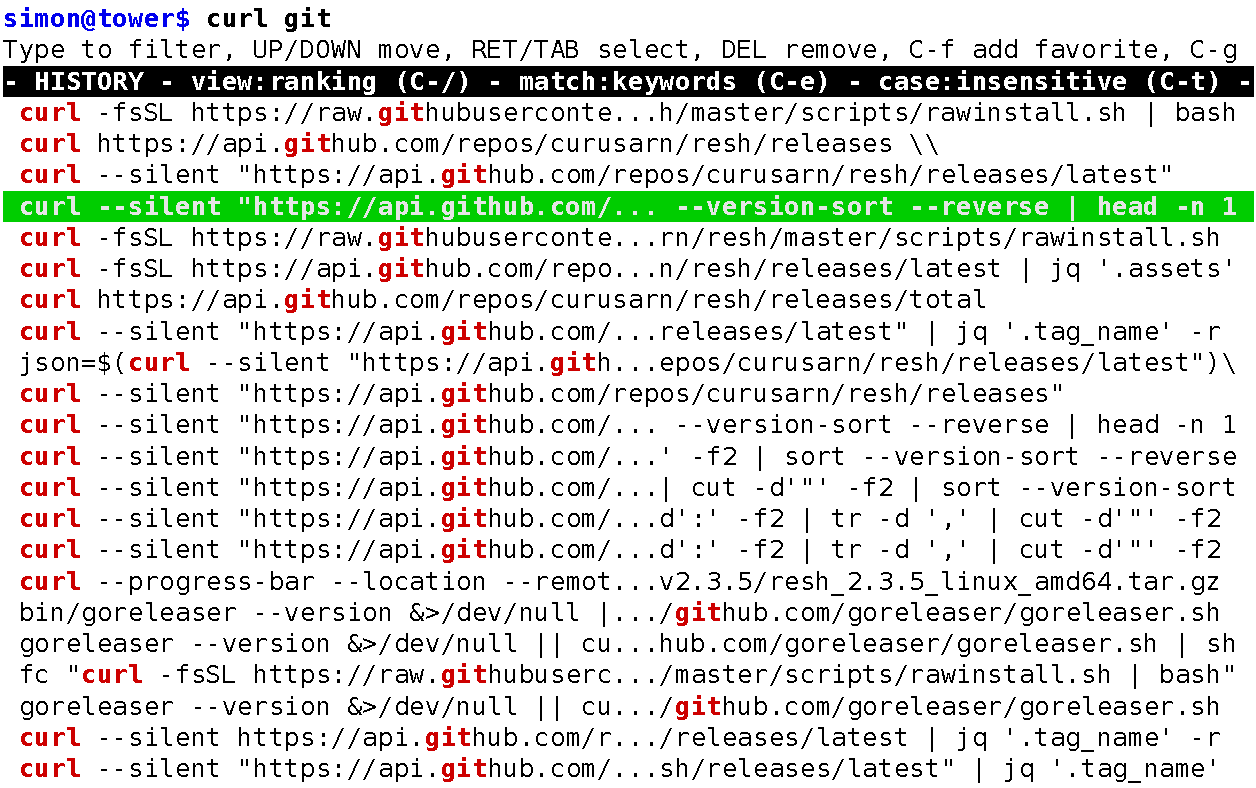
\includegraphics[width=0.995\linewidth]{figures/existing-tools/xterm-hstr-std.pdf}}
  \caption{Hstr interactive history search}
  \label{hstr-screenshot}
\end{figure}


\subsection{Fuzzy history search}

Fzf\cite{tools-fzf} is a popular\footnote{Fzf has over twenty eight thousand "stars" on GitHub.} general-purpose command-line fuzzy finder. The documentation of the project recommends several ways that can be used to interactively search shell history.

Searching history using Fzf addresses the issues of the history reverse search. 
Like Hstr, Fzf can display a full page of results from history. 

Fuzzy search allows Fzf to retrieve both exactly and approximately matching history entries. Exact and close matches are returned first and additional matches are returned after. 

This essentially provides a functionality of multi-query search. In addition, fuzzy search can match the desired history result even when you make typos in the query. Unlike "keywords" matching, fuzzy matching is tolerant to mistakes and typos; Naturally, this is very appealing to users. 

Fuzzy search is a commonly requested feature in various history tools. Some people who are already using Fzf cannot imagine using history tools without fuzzy search.

% \begin{figure}\tmpframe{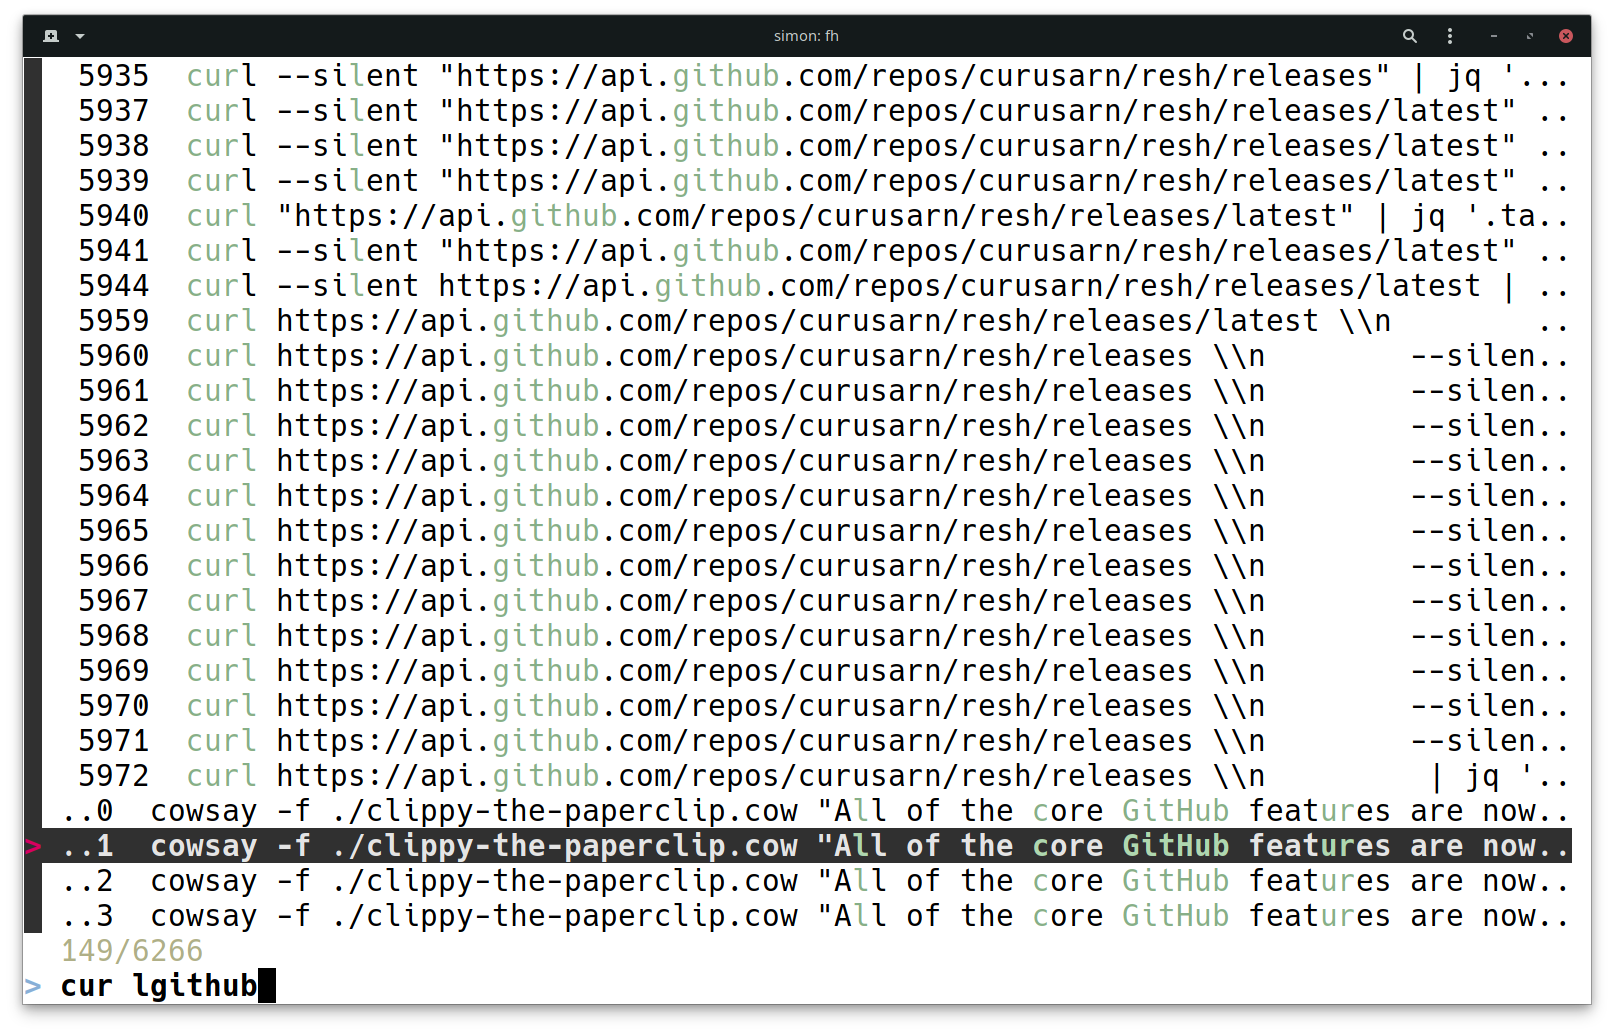
\includegraphics[width=\linewidth]{figures/existing-tools/fzf-fh-screenshot.png}}\caption{Searching history interactively using Fzf}\end{figure}

\begin{figure}
  \permanentframe{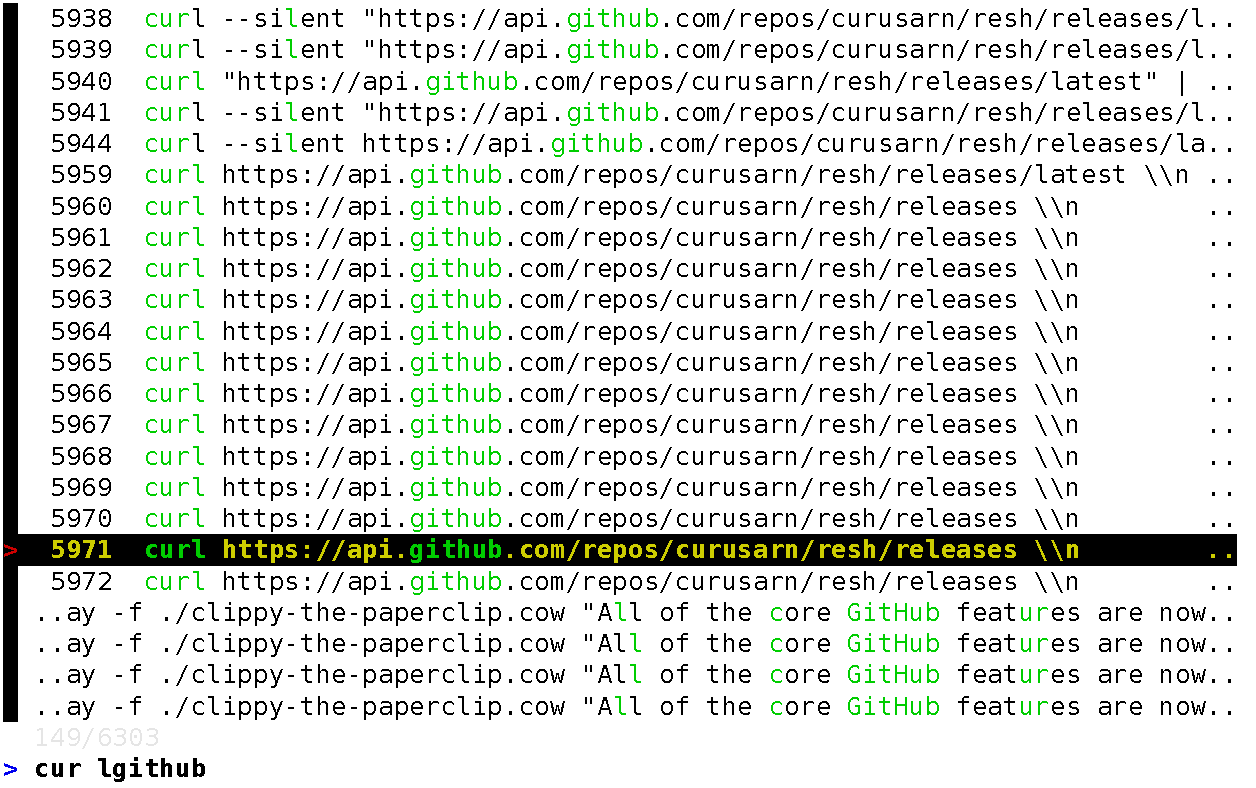
\includegraphics[width=0.995\linewidth]{figures/existing-tools/xterm-fzf-std.pdf}}
  \caption{Searching history interactively using Fzf}
\end{figure}


%\subsection{Per directory history}

%The idea behind per directory history is that your history is grouped based on directories. In practice, this means that each directory has a separate history file. 
%Since this is reasonably easy to set up, we can find many mentions, configurations, and even smaller projects that do save history to a separate file for each directory.


%Different smaller projects
%People do this even when it means not being able to reverse search the entire history.

%% https://github.com/jimhester/per-directory-history  123 gh stars
%provides switching (keybinding) between global and directory history


\subsection{Contextual shell history in the cloud}


Bashhub\cite{toolsbashhubclient} saves your shell history to the cloud and allows you to search it from all of your machines.

Apart from the command line entry, Bashhub records and saves additional context. Each history record contains following:
\begin{itemize}
    %\setlength\itemsep{0em}
    \item command line entry
    \item exit status
    \item present working directory
    \item host
    \item time of execution
    \item ID of the session
    \item ID of the record
\end{itemize}

The Bashhub history search uses pattern matching\footnote{The pattern matching is implemented using SQL "LIKE" operator.} to search the submitted command line entries. The search can be restricted to current directory and to current host.


All searching is server-side; This means that every time you search your history using Bashhub it needs to send a requests to a remote server.
These requests take time so there is no interactive "search as you type" functionality. Instead, you always have to type out the full query, execute the search command, and then wait%\footnote{Bashub server response takes about three seconds on my system.} other 
for the results. Below, you can see an example of search command that is restricted to the current directory. 

\begin{verbatim}
    bh -d "curl git"
\end{verbatim}

An obvious disadvantage of server-side search is that it does not work offline. 
When you use Bashhub, your history is saved on the remote server and the server needs to be able to search it. This means that the history is on the server, at least in memory, in an unencrypted form. Adding client side encryption would break the server-side search.

By default, the remote server is an instance maintained by the project author. The official server implementation is closed source. This means that you need to trust the author of the project with the access to your shell history. 

Recently\footnote{Open source implementation of Bashhub server was written in February 2020.} a new open source implementation\cite{toolsbashhubserver} of the Bashhub server has appeared. This addresses the privacy and security issues by making it possible to run and use your own instance of the server.

\redtext{Bashhub is somewhat popular on GitHub\footnote{Bashhub has 744 "stars" on GitHub.}
Bashhub is not a viable replacement for standard reverse search and manual history searching.}

%ALT sample: There is an additional open source implementation of Bashhub server available.
%ALT sample: This makes it possible to self-host instead of trusting the someone with your shell history.


% bashhub library
\redtext{Mention https://github.com/rcaloras/bash-preexec library ??? I don't think so}

\subsection{Contextual history search powered by a neural network}

McFly\cite{toolsmcfly} is a tool that tries to predict your next command line entry using a small neural network. It predicts the next command line entry based on following contextual information:
\begin{itemize}
    \item present working directory
    \item previous command line entries
    \item how often you run the command line entry
    \item the last time you ran the command line entry
    \item if you selected the command line entry in McFly before
    \item exit status
\end{itemize}

Unlike Bashhub, this tool is designed to be bound to \verb|CTRL-R| and to replace the standard reverse search. Pressing \verb|CTRL-R| launches McFly full screen terminal app shown in figure \ref{tools-mcfly}. At first, the app displays a list of ten predicted history entries. The list of history entries is updated as you type to only show results that exactly match the typed query. The list always contains ten results or less which is a curious design decision. 


\begin{figure}[h]
  \permanentframe{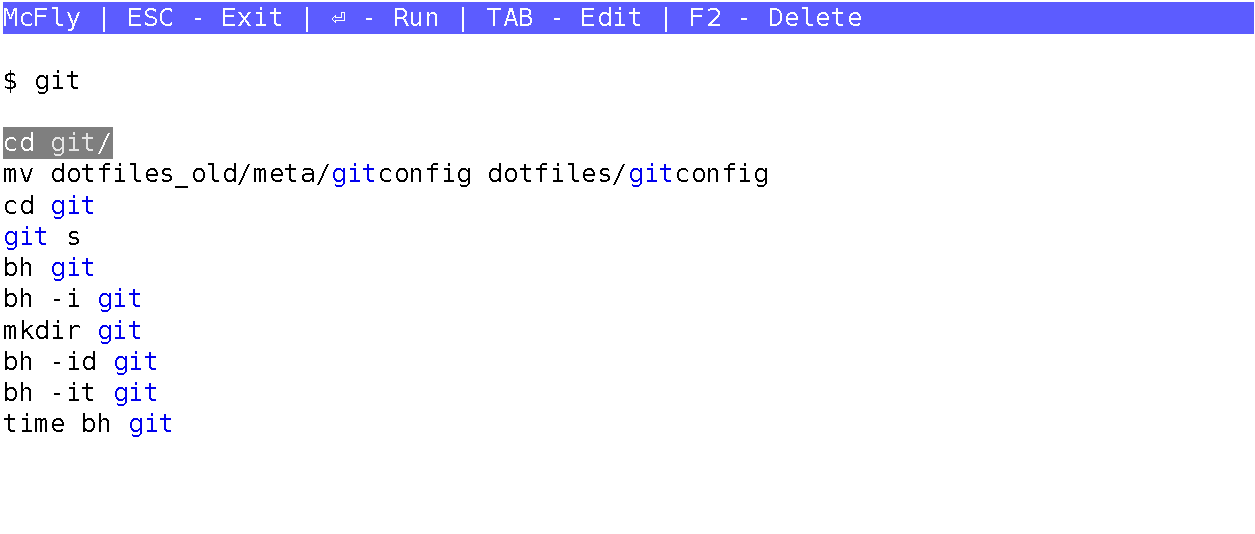
\includegraphics[width=0.995\linewidth]{figures/existing-tools/xterm-mcfly-std-short.pdf}}
  \caption{McFly interactive history search (cropped)}
  \label{tools-mcfly}
\end{figure}


When trying to use McFly we found its behavior to be unpredictable; Not knowing why specific results are being shown made the tool less useful. 

McFly also shares some problems with reverse search, it only uses a single query for searching; This can make it hard to find what you need in situations when you are unable to think of a better query\footnote{We already described such situation in \redtext{REF: reverse search workflow}}. 

\redtext{McFly is popular on GitHub.\footnote{McFly has about sixteen hundred "stars" on GitHub.}}

%\begin{figure} \permanentframe{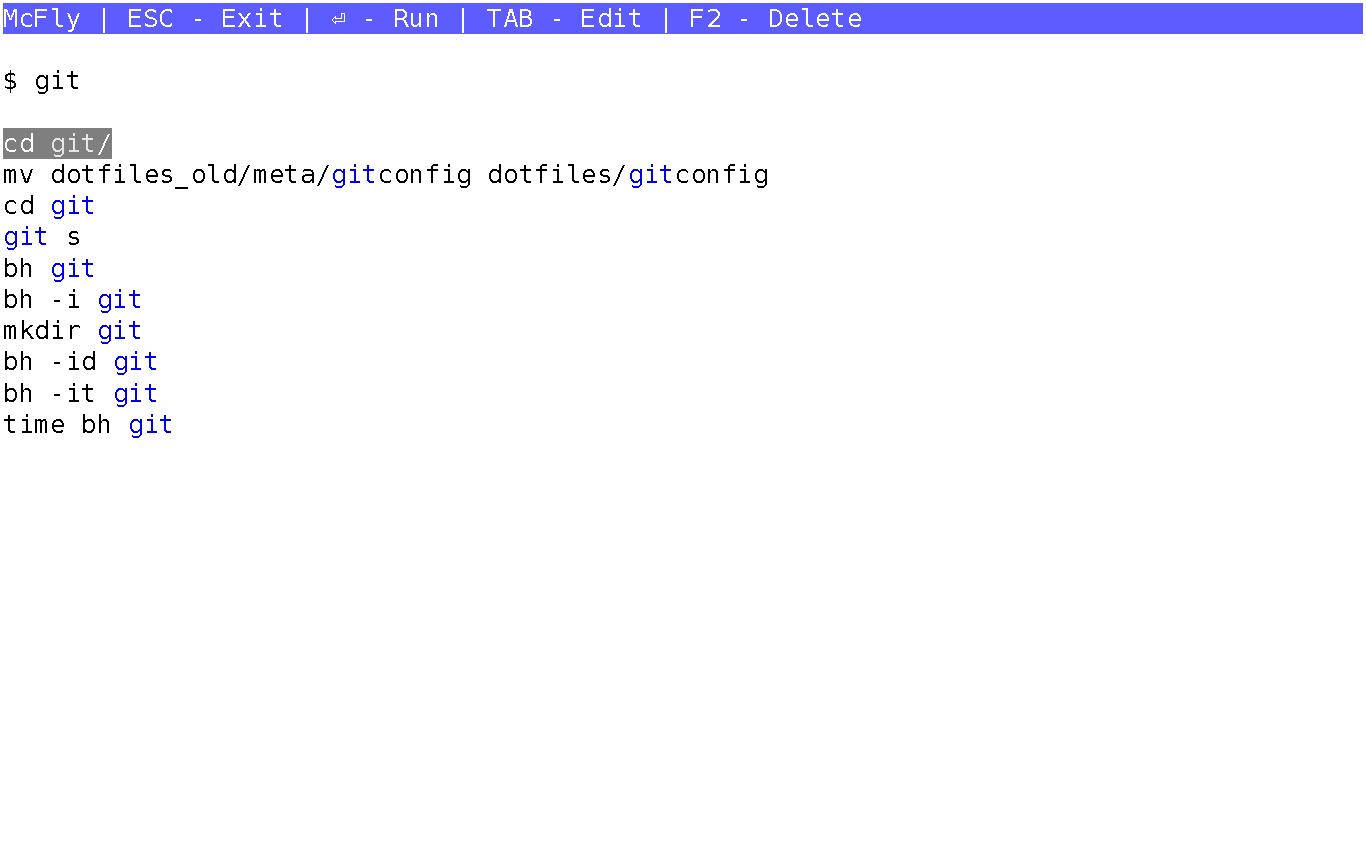
\includegraphics[width=0.995\linewidth]{figures/existing-tools/xterm-mcfly-full.pdf}}  \caption{McFly interactive history search \redtext{REMOVE IMAGE}} \end{figure}


\todo{DELETE this section vvv}

\subsection{Contextual history saved in a SQLite}


\redtext{TODO: advanced-shell-history - contextual history with smart querying - too buggy to be useful - non-interactive}



\todotext{TODO: Other less notable shell history tools - underdeveloped, non-interactive, ...}
% https://github.com/larkery/zsh-histdb  608 gh stars +it is a oh my zsh plugin


%%%
these tools usually store the history in a SQLite database. This makes sense because the history is inherently relational. However, this can potentially limit the ability to use regex or fuzzy searching. This must not be underestimated given how popular and powerful fuzzy searching is. 
% is this desing? ^^^


\paragraph{}

\redtext{TODO: short conclusion about history tools, configurations, etc.}


%\redtext{Explicit searching by context sounds like a useful feature obvious feature for tools that record history with context. 
%While this feature is easy to implement and it sounds useful it does not really bring much value. }


\redtext{Hstr and Fzf are a major improvement over standard history reverse search. Bashhub and McFly use context but they do not match the benefits provided by Hstr or Fzf. }

There are some tools that did not warrant a separate section. 

These tools provided features like explicit history search.
%\redtext{There are other contextual history tools. Usually, they save some basic context like directory and exit status to a SQLite database. The main feature of these tools is the ability to explicitly search history by context. }

\redtext{All of these contextual tools show us that it is not easy to use context in a meaningful way. We should carefully examine the available context and consider how it can be useful to the user.}

\section{Usefulness of contextual information}

% rewrite

In previous section we talked about existing history tools. We saw that contextual history tools are not automatically more useful than tools that do not work with additional context. 

Useful history tools address real workflows and provide value to the user.
In this section, we explore available contextual information. We will discuss how different parts of the context relate to shell usage and history usage. %We do this to identify the usefulness of different parts of available contextual information. 

\redtext{IDEA: a bulleted list of the 5 following sections}

\subsection{Exit status and pipestatus}

Zero exit status is interpreted by the shell as success; In contrast, non-zero status indicates failure.\cite{bashman} People often immediately edit and resubmit command line entries that returned an error. However, people probably rarely want to repeat older command line entries that failed. Does this mean that we can use exit status to filter out errors and only serve successful history entries to the user?

Not really, exit status does not directly map to success and failure. Programs can fail without returning an error. Some programs return non-zero exit status without actually failing\footnote{For example, GNU Grep returns one when no lines were matched and two to indicate errors.\cite{man-grep}}. 
Additionally, even history entries that are technically errors can be useful to the user. For example, the user might interrupt a program using \verb|CTRL-C| after it has fulfilled its purpose.
% We could ADD: logical errors

Generally, it is reasonable to assume that people retrieve history entries with zero exit status more often than the ones with errors. However, given the caveats described above, we should excercise this assumption conservatively. Removing history entries based on exit status would prevent the user from retrieving them. To preserve this ability we can display all history entries but prioritize the successful ones.


In addition to exit status, there is \verb|$pipestatus| shell variable. Pipestatus gives us additional information about exit status of commands in a pipeline; Pipeline is a sequence of commands connected by shell pipes. Pipestatus is an array of exit statuses of individual commands that make up the pipeline.\cite{bashman}\cite{zshdocs} Pipelines that return zero exit status can still contain failed commands\footnote{\redtext{pipefail (both bash and zsh)}}. History entries with even one failed command in the pipeline can be treated as unsuccessful.
 
%PIPESTATUS (bash)
%An array variable (see Arrays) containing a list of exit status values from the processes in the most-recently-executed foreground pipeline (which may contain only a single command).

%pipestatus <S> <Z> (zsh)
%An array containing the exit statuses returned by all commands in the last pipeline.

\subsection{Directory and Git related context}

Directories provide explicit context; People change into different directories to complete different tasks.\cite{greenberg1993computer} It is often more comfortable to change directories compared to using longer paths as arguments. 

Many standard tools encourage the user to use specific directories for specific tasks. 
For example, Makefile, Vagrantfile, and Dockerfile are all designed to be used from within their directory\cite{man-make}\cite{docs-vagrantfile}\cite{docs-dockerfile}. 

Directories often hold projects that are associated with specific workflows and command line entries. 
These projects often use Git or other version control system; This almost forces the user to use command line entries specific to the project inside the version control repository. 

We should make it easy to access the history entries from the present working directory.
However, we do not have to stop there. Directories and Git repositories are closely related but they are not quite equivalent. Git provides some more context we can use. 
%The goal is to differentiate between history entries executed inside and outside the Git repository. 
Root of the Git repository allows us to group all history entries from the Git repository.
Git remotes\footnote{Remotes are remote repositories tracked by Git. Origin is the default remote.} can be used to identify the repository even across different machines or when it is moved to a different directory. 




\subsection{Sequential relationships, sessions, and time}

% In this section, we cover a part of context that is not well understood yet. captur

Command line entries are generally not executed individually; They are a part of longer sequences and tasks.\cite{greenberg1993computer} Each entry is related to its preceding and following command line entries. 

In previous analysis\redtext{REF: dependencies between commands }, we saw that there are sequential dependencies between command stubs; These dependencies represent workflows that users recognize and remember.

Apart from immediate sequential dependencies, each command belongs to a terminal session\footnote{\redtext{???} Terminal session consists of all history entries entered into the same terminal. Terminal sessions are equivalent the shell sessions in the majority of cases.}. Our data shows big differences between how people use sessions; Some people often create new terminals even for a few command line entries and then close them. Others keep terminals open for a long time and reuse them for different tasks.
Additionally, people very often switch back and forth between multiple open terminals. Command line entries from simultaneous terminal sessions are usually different but all related to the same task.

These relationships between history entries and sessions are definitely interesting and possibly useful. To illustrate, imagine you type a command line entry that you already executed five times in the past. Maybe it is related to a specific task and to complete it you will need similar commands as before. Situations like this one show us the potential usefulness of session and history entry relationships.

However, it is not obvious if these relationships are general enough to be useful in the average case. It is unclear how to use this complex contextual information to provide value to the user. It is beyond the scope of this work to study the relationships between history entries and between sessions.


Nevertheless, not all of the sequential contextual information is difficult to interpret and use. Sequences of history entries are useful because there are situations when people want to repeat them\footnote{We saw such situation in section \ref{workflow-repeating-a-sequence} earlier}. We should support such workflows.
%Since sequences of history entries are directly related to a workflow we identified earlier\redtext{REF: sequential workflow} we should use the sequential property in our design. 

One more use for sequences of command line entries is recording them as a full non-deduplicated transcript. Having a full transcript of your actions gives you the ability to refer back to what you were doing earlier. A transcript of command line entries should also include the time of execution for the individual entries.
% NOT an auditing tool

%Having access to a full sequential history\footnote{Standard shell history is often deduplicated. Full sequential history is a shell history that is not deduplicated.} that represents a transcript of your actions also has its value.

\subsection{Host and portability of history entries between devices}

Imagine that you have your shell history synchronized between multiple devices.
Each of the devices is at least a little bit different so it is a good idea to be able to tell them apart. The \verb|$HOST| environment variable is a good identifier of the device. 

Since each device can be different we should look at the possible differences that are relevant to the shell history. Different operating systems\footnote{We are only considering Unix-like systems in this work.} use different package managers to install software. For example, Debian-based distributions use Apt, Arch-based distributions use Pacman, and on MacOS people use Homebrew. Commands for one package manager will not work with others.

Many history entries are valid in both Bash and Zsh but not all history entries. Shell configuration might differ between devices which could cause some history entries to not work on all devices properly. A good example are specific shell aliases that the user added to one of their devices.

% installed software

We just described why some history entries will not work when executed from a different device. Some history entries might not work even when executed on the same device but out of the original context. Examples of this are shell variables and relative paths; Variables that were set at the time of execution can cause history entries to fail when retrieved and executed again. History entries with relative paths will only work in certain directories.

As we can see there are many reasons why history entries might not be portable. Most of the issues above can be detected using relevant contextual information. 
We could detect and handle these portability issues individually. Or alternatively we could take a simpler approach; Prioritize history entries from the current device over those from other devices. This could be effective because many of the portability issues are related to mixing shell history from different devices. 


%We can use the host to prioritize the history from the current device and to explicitly show the user which host is the specific history entry coming from.

\todo{NOTES related to compatibility - might be useful later in the design chapter}

%However, only some of these portability issues have elegant solutions. For example, aliases can be detected and saved as part of the history entry. Upon retrieval the user can get an offer to set the alias or to even add it to the shell RC file\footnote{RC files for Bash and Zsh are ".bashrc" and ".zshrc" respectively.}. 

%penalize
%warn
%bundle and restore

%We could use this information to detect and handle these situations. warn the user or even bundle and recreate the original context. 

% Understanding the command line entry is hard  
% Modifying the command line entry is hard

% Understanding limited parts of the command is doable  
% Recreating the context of the command is doable  
% -$>$ Bundling the context with the command is doable

% Imagine a command with relative paths and two approaches: 1) you modify the paths to be absolute and then somehow offer the modified command to the user 2) you detect the presence of relative paths and offer an option to change to the directory on recall

\subsection{Usage of history mechanisms}

So far we have only described context related to the the usage of shell and to the device. Now we look at context that is related to how people use shell history. 

The first step is to know which command line entries are typed and which are retrieved from history. Next, it would be useful to know which history mechanism was used to retrieve the entry. This information is useful because people tend to repeat themselves. 
For example, when you retrieve a specific history entry using \verb|CTRL-R|, you are more likely to retrieve it using \verb|CTRL-R| again in the future. %This is supported by previous research; According to Greenberg, it should be it easy to retrieve history entries that were already retrieved earlier.\cite{greenberg1993computer}


A detailed transcript of user interactions with the history mechanisms would give us even more useful information. Consider a situation where the user presses \verb|ARROW_UP| ten times and then gives up and uses \verb|CTRL-R| to search the history instead. This is not an effective way to use history. However, it would be wrong to blame the user. If such situation happens a lot to many users we should look into if we can redesign \verb|ARROW_UP| to improve it.

From the perspective of User-centered design, the interaction between the user and the history system is everything. It is essential for informing design decisions and estimating usefulness of the system. Interactions can help us understand when the system works and when it does not.
 
When exploring relevant research, we did not find anyone who recorded shell history with the history interactions of the user. Furthermore, we did not find any tools that are capable of recording the shell history with user interactions. We think that collecting a dataset of shell history with the user history interactions would enable future research. To move forward towards this goal we should record the history usage data as part of the history.


% DESIGN NOTES

\todotext{XXX: Guidelines to mention/cite in the text}

\todotext{Response times - usability}

https://www.nngroup.com/articles/response-times-3-important-limits/

0.1s - “system is reacting instantaneously” -$>$ prompt - recording

1.0s - “user's flow of thought to stay uninterrupted” -$>$ cli app prototype maximum load time

10s - ...
\todotext{Visibility of system status}
X1: Visibility of system status
system should communicate its state -> highlights, all info displayed
challenge with more underlying info

\todotext{X4: Consistency and standards}

\todotext{Discoverability}

bad in shell

related: recognition rather than recall, consistency and standards
important for user experience, adoption, learning curve
generally hard in shell (recall-based)
-$>$ don’t break expectations (conform to standards)
e.g. new keybinds are not a great idea
make use of habits people could already have built while using std shell history features
e.g. people use arrows to get recent commands and ctrl-R to get arbitrary commands

\todotext{Minimal, simple}

guideline from NNgroup

“Overloading a reuse facility with complex functionality would not make it better.” greenberg


\chapter{Design}

\subsubsection{Recording user interactions}

\redtext{good text - bad place - maybe move up? - (this is "UP")}

During working on this project we did encounter a lack of tools that can be used to record interactions between the user and the history system.
User interactions are essential for understanding usage patterns and for informing design decisions.
We want our tool to record user history interactions.
This should enable more future research of how people use shell history.

\redtext{Lorem ipsum dolor sit amet, consectetur adipiscing elit, sed do eiusmod tempor incididunt ut labore et dolore magna aliqua. Ut enim ad minim veniam, quis nostrud exercitation ullamco laboris nisi ut aliquip ex ea commodo consequat. Duis aute irure dolor in reprehenderit in voluptate velit esse cillum dolore eu fugiat nulla pariatur. Excepteur sint occaecat cupidatat non proident, sunt in culpa qui officia deserunt mollit anim id est laborum.
Lorem ipsum dolor sit amet, consectetur adipiscing elit, sed do eiusmod tempor incididunt ut labore et dolore magna aliqua. Ut enim ad minim veniam, quis nostrud exercitation ullamco laboris nisi ut aliquip ex ea commodo consequat. Duis aute irure dolor in reprehenderit in voluptate velit esse cillum dolore eu fugiat nulla pariatur. Excepteur sint occaecat cupidatat non proident, sunt in culpa qui officia deserunt mollit anim id est laborum.
}


\todotext{Write intro}
In this chapter we design our history system

before jumping into the design itself we want to point out a few pieces of information that motivate our decisions.


People are used to standard history features

we should not redesign them unless we have a good reason to

furthermore, even when we redesign and replace history features we should leverage and build upon habits people already have.



\section{Requirements and features}


The requirements we selected based on the previous analysis are following:

\begin{itemize}
    \item Record shell history with context and usage
    \item Allow unlimited history
    \item Allow history sharing between open sessions
    \item Provide good out-of-the-box experience (too high-level?)
    \item Respect existing habits of people (too high-level?)
    \item Provide a replacement for reverse search
    \subitem Solve the issues with standard reverse search
    \subitem Match the improvements offered by Hstr and Fzf
    \subitem Use recorded context to enhance history searching capabilities
    \item Provide support for sequence repeating (forward in history)
    \item Provide support for synchronization of shell history between devices
    \item Provide support for contextual autosuggestions
\end{itemize}



\subsection{Basic features}

Now, we describe the basic features of the design. These features might seem obvious but we point them out because they do contribute the resulting usefulness of the history system.

History should be collected and recorded in a robust way; History should be unlimited, and using multiple simultaneous sessions must not result in missing history entries. All this has to work by default; No configuration should be necessary to achieve the basic functionality. 

Default configuration should provide good out-of-the-box experience for the average target user. 
Simultaneous sessions should be handled is a way that allows accessing history from other sessions.


\subsection{Core features}

The core focus of this design is providing a replacement for the standard reverse search. In this section, we explain why we chose this as the main focus of the design. We discuss how it relates to standard shell history features, existing state-of-the-art history tools, and possibilities of enhancing history searching with context.

\todo{remove the paragraph titles?}

% These features address the most common workflows and the most significant shortcomings of standard history.

%We are differentiating between the core features and additional features because it is important to keep the scope of the project tight.
% even when there are additional features that would work well with it.

\paragraph{Standard history features}

Standard history features form the base that people are used to. We should not redesign and replace them unless we have a good reason to.
As we saw in analysis, standard reverse search does not provide a good feature set to complete many workflows. Furthermore, there are other tools available that provide features that solve the issues of reverse search. Because of this, we design a searching application that replaces and improves the reverse search.

%For example, we have no reason to change history expansion. Accessing recent history entries using \verb|ARROW_UP| works reasonably well in many situations. Furthermore, people expect \verb|ARROW_UP| to give them immediately previous history entries. Because of these reasons we do not redesign \verb|ARROW_UP|.

% In contrast

\paragraph{Matching the state-of-the-art}

Hstr\cite{toolshstr} and Fzf\cite{tools-fzf} are existing projects that replace reverse search and provide improved searching capabilities. 
Standard reverse search only uses a single query for searching and displays a single result at a time. In contrast, both of the tools mentioned above allow using more than a single query for searching and show a full screen of history results. We use these tools as an inspiration. Our searching application should match the improvements provided by Hstr and Fzf. 

\paragraph{Enhancing history searching with context}

%In analysis, we have identified workflows which are directly related to context. 
%Additionally, we described different ways how context relates to shell usage. 

In addition to matching the state-of-the-art features, we want to use context to enhance the searching capabilities of our history system. Our searching application should make it easier to retrieve history that matches the current context. 
% todo: do not be as specific CUT here


%This means that history entries from current directory, git repository, and host should be prioritized.
%In contrast, history entries with errors should be penalized.
%The relevant context should be visible when it affects the order of results.
%However, the user interface should not be cluttered with irrelevant context. 



\subsection{Additional features}

In this section, we cover features that are not the main focus of our design. These features are less important in comparison to providing a replacement for the reverse search. However, they are still valuable and we want to make sure they fit with with the rest of the design. 
The chosen additional features are Forward in history, synchronizing history between devices, and Fish-like Autosuggestions.



\paragraph{Forward in history}

Forward in history is a feature we can find in Python console in Blender. We adopt this feature into our design because it allows the user to easily repeat sequences of history entries. Support for repeating sequences from history is poor in standard shell history.

\paragraph{Synchronizing history}

Synchronizing history between multiple devices is and appealing feature. It enables history reuse between devices. The potential for reuse is further enhanced by using context to prioritize the search results.
Synchronized history is also harder to lose because it is replicated across multiple devices. 

\paragraph{Autosuggestions}

Autosuggestions are a very convenient and very fast history mechanism. Original Fish autosuggestions use context to determine what history entry should be displayed.
We want to include a similar feature in our design.

\section{Architecture}

In the previous sections, we listed all the features that we chose to include in the design. We chose a set of features that fits well together and should significantly improve the usefulness of shell history.

Now, we design the architecture of our history system so that it can accommodate all the features. 
Our history system consists of a daemon and multiple components. The daemon is always running in the background and components are integrated into the shell and activated at appropriate times. 

%\paragraph{Daemon}

Daemon allows us to asynchronously preprocess the history data and serve it to the components when it is needed. It is responsible for loading and saving history to the storage. Daemon gives us the option to easily share history between sessions. History synchronizations is initiated and controlled by the daemon.

%\paragraph{Components}

There are multiple different components which are activated at various times based on their purpose. History collector records the shell history with context and sends it to the daemon. Autosuggestion and arrow keys handlers respond to the interactions with the user. Finally, the search application interacts with the user, communicates with the daemon and also does its own share of data processing.


For the purpose of this design, we divide the system into two logical sections - frontend and backend. As you can see in the figure \ref{design-architecture-layers}, frontend is responsible for the interactions with the shell, terminal, and by extension the user. Backend is mostly about handling data. 

\begin{figure}
\centering
  \tmpframe{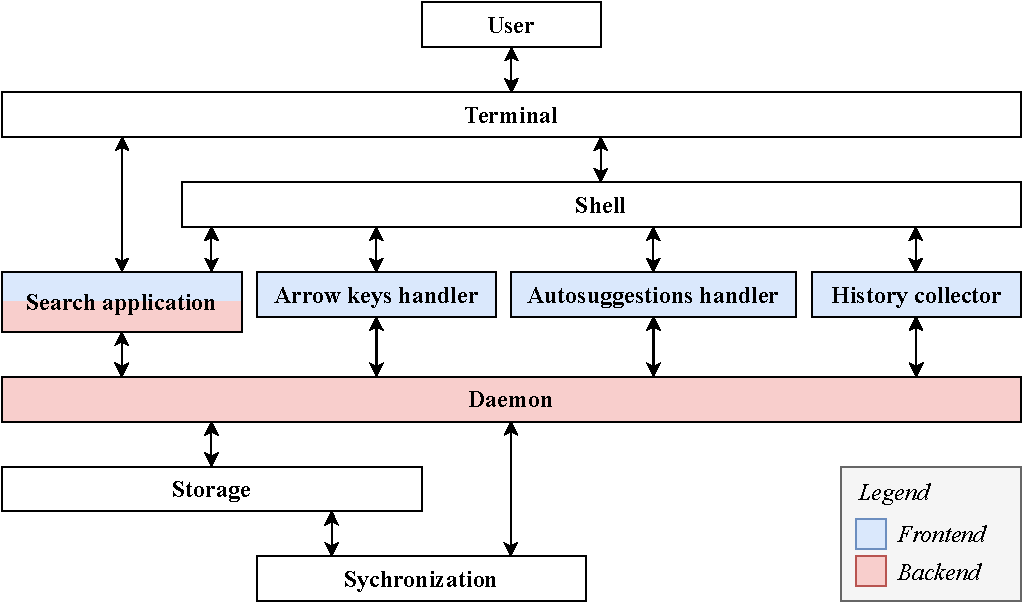
\includegraphics[width=\linewidth]{figures/design/thesis-design-architecture-layers-v2.pdf}}
  \caption{Schema of architecture and communication}
  \label{design-architecture-layers}
\end{figure}

\section{Frontend}\label{design-frontend}

In this section, we focus on and design the parts of that system that the user interacts with. 
To relate this to our previous analysis, these are the specific workflows we are addressing in this section:

\begin{itemize}
    \item Searching with limited knowledge (section \ref{workflow-search-w-limited-knowledge})
    \item Searching with implicit context (section \ref{workflow-search-w-implicit-context})
    \item Repeating a sequence of history entries (section \ref{workflow-repeating-a-sequence})
\end{itemize}

\subsection{Search application}

The most important part of our design is the replacement for standard reverse search - a full-screen terminal history searching application. The application is inspired by Hstr and Fzf. 

We start by designing the visual layout of the application.
Wireframe in figure \ref{wireframe-normal} shows the layout of the default view of the application. There are three sections in the wireframe:

\begin{itemize}
    \item Search input
    \item Main section with search results
    \item Status bar with details and help
\end{itemize}

The search results in the main section are interactively updated as the user types into the search input. 


\begin{table}[]
\centering
\begin{tabular}{lllll}
\hline \hline
Sample name             & \multicolumn{2}{c}{Recurrance rate} & \multicolumn{2}{c}{Range} \\
                        & mean             & std dev          & minimum     & maximum     \\ \hline
Novice Programers       & 80.4\%           & 7.2              & 64.7\%      & 91.7\%      \\
Experienced Programmers & 74.4\%           & 9.7              & 51.4\%      & 90\%        \\
Computer Scientists      & 67.7\%           & 8.2              & 46.4\%      & 82\%        \\
Non-programmers         & 69.4\%           & 8.1              & 50\%        & 84.3\%      \\
                        &                  &                  &             &             \\
Total                   & 73.8\%           & 9.6              & 46.4\%      & 91.7\%      \\ \hline \hline 
\end{tabular}
\caption{The average recurrence rate of the four sample UNIX user groups from \cite{greenberg1993computer}}
\label{tab:recurrence_rate}
\end{table}

\begin{table}[h]
\centering
\begin{tabular}{lllll}
\hline \hline
context        & header       & visible                             \\\hline
time/date      & TIME         & always                              \\ 
host           & HOST:        & only for history from other hosts   \\ 
directory      & DIRECTORY    & always                              \\ 
git repository & FLAGS*       & only for history from this git repository \\ 
exit status    & FLAGS*       & only non-zero exit status           \\ 
command line   & COMMAND-LINE & always                              \\\hline \hline
\end{tabular}
\caption{Context and columns in the default view}
\caption*{\footnotesize *git repository and exit column share the same header}
\label{tab:design-columns}
\end{table}


Command line entry, directory, and time are always displayed but they are shortened to fit the screen. Other information is only displayed when relevant to not clutter the view and to save space.

Near the bottom of the screen there are details for the currently selected command. These include various information about the command without any shortening.


\begin{figure}
  \permanentframe{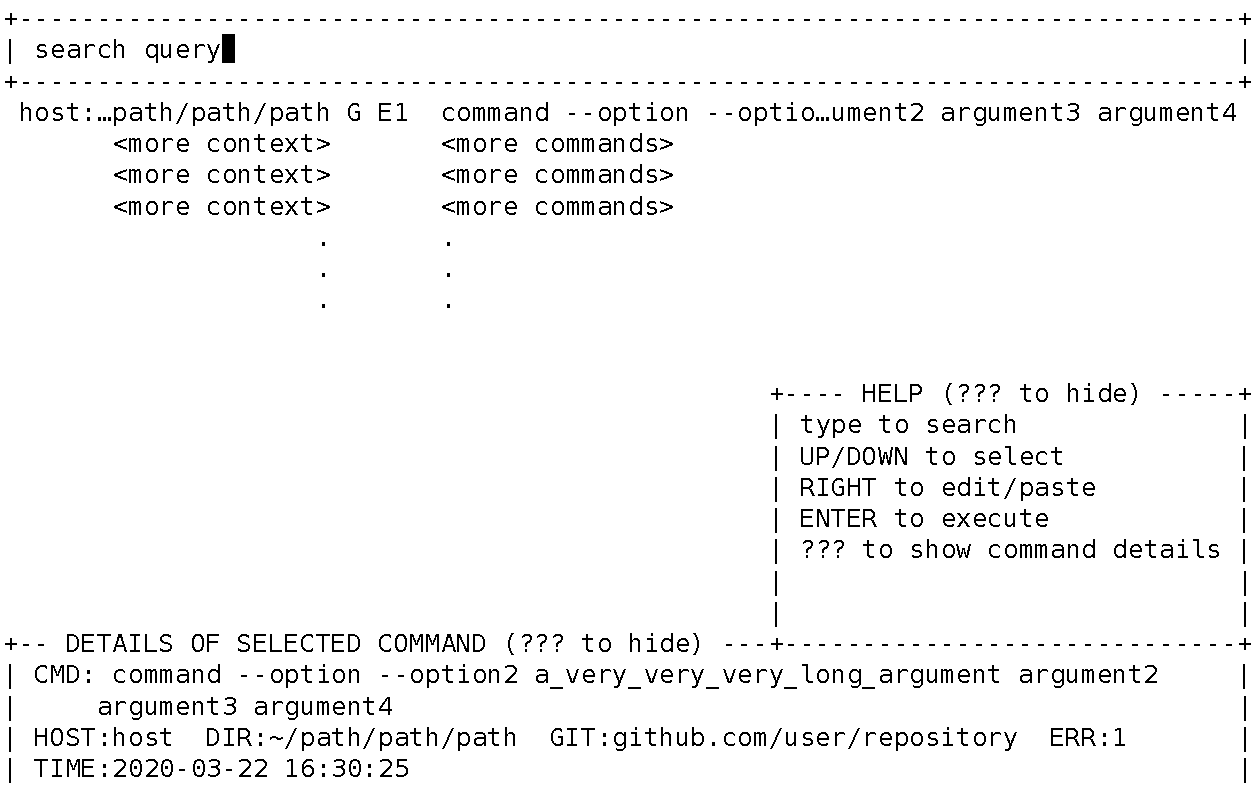
\includegraphics[width=0.995\linewidth]{figures/design/xterm-wireframe-bw-normal.pdf}}
  \caption{Wireframe of default view}
  \label{wireframe-normal}
\end{figure}

The wireframe in figure \ref{wireframe-detail} shows the detail view. In this view the user can see the details and surrounding history entries for a single command line entry. Each command line entry can appear in history multiple times; The user can switch between these occurrences. The next occurrence is partially displayed to make it easier to list and compare the surrounding history entries.

\begin{figure}
  \permanentframe{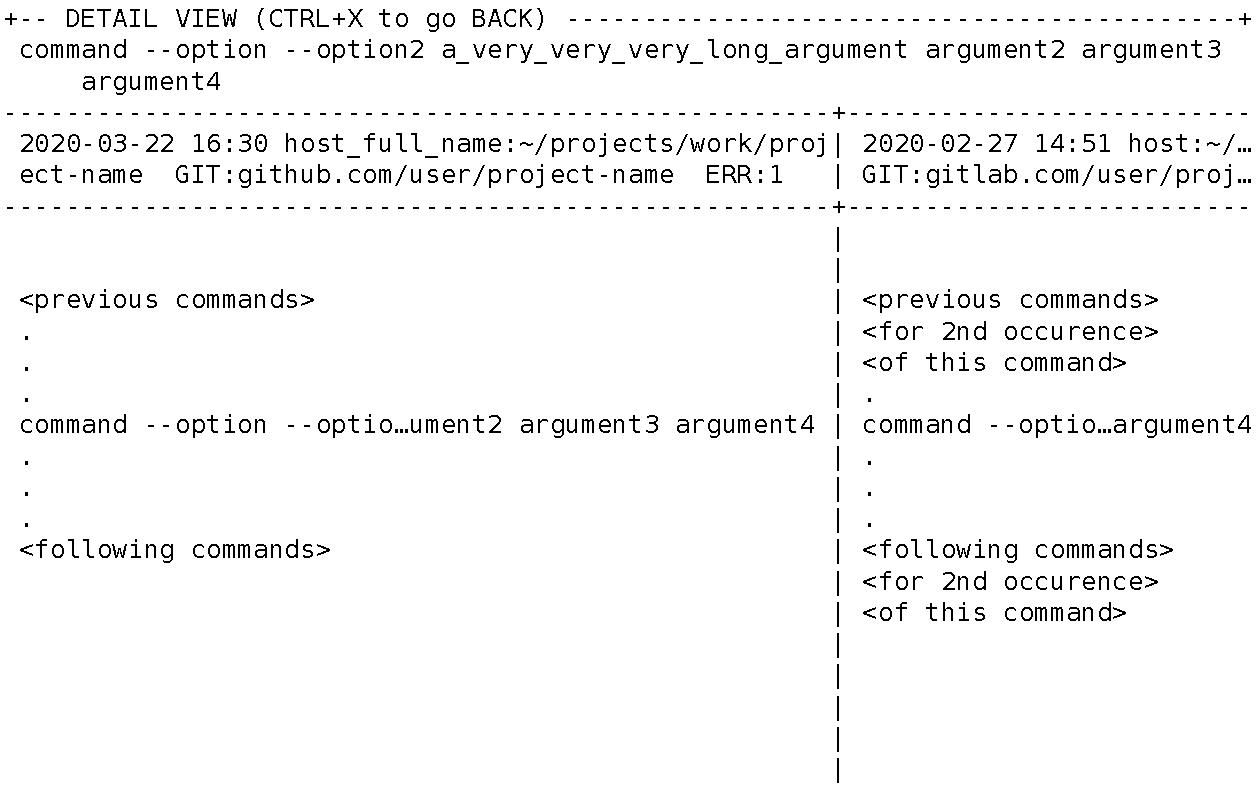
\includegraphics[width=0.995\linewidth]{figures/design/xterm-wireframe-bw-detail.pdf}}
  \caption{Wireframe of detail view}
  \label{wireframe-detail}
\end{figure}



% \subsubsection{Modes (Context/RAW)} - added after user feedback

\subsubsection{Key bindings}

Since we are aiming to redesign and improve the reverse search we replace its key binding; Pressing \verb|CTRL-R| launches our search application instead of the reverse search. CTRL-S is intentionally left without function to avoid collisions with control flow key binding. % + other keys we want to avoid
To not force the user to learn new key bindings we use similar key bindings as the reverse search. Typing searches and filters the results. % CUT HERE 
Arrow keys (\verb|UP|/\verb|DOWN|) are used to select history entries. Pressing \verb|ENTER| executes the selected entry. Pressing \verb|ARROW_RIGHT| pastes the selected entry onto the command line to allow additional editing. The application can be closed with \verb|CTRL-C| or \verb|CTRL-D|.

We chose new key bindings for features that are not present in the reverse search.
Pressing \verb|CTRL-E| switches between the default and the detail view.
Help can be toggled with \verb|CTRL-/| and details section can be toggled with \verb|CTRL-T|.

\redtext{Shorten}

\redtext{consistently take inspiration from emacs}

\subsubsection{Design from 80x25 to fullscreen}

Wireframes above both use standard 80x25 character terminal size. In larger terminals there is more space that can be used. Directories and command line entries stretch. A new column with time of execution appears on the left. The master section becomes longer and as a result more history entries fit in the terminal.   

\subsubsection{Colors}

Our application has a lot of information to display. 
Colors will be used to highlight the information that influences the order of displayed results. To make it easier to differentiate between different types of information they will be highlighted using different colors. 
Red color will be reserved for highlighting remote hosts and non-zero error status; This communicates to the user that these history entries might not work well.
Currently selected history entry will be highlighted by inverting the foreground and background colors.

\subsubsection{Customizability}

\redtext{Defaults matter a lot because most people will not change them.}

\subsection{Arrow key handler}

In this section, we design the behaviour of features that are available while on the command line. We introduce minor changes into the standard behaviour.

\subsubsection{Prefix search}

In our design, prefix history search is enabled by default. It is a useful feature that does not interfere with the standard stepping through history. 

\subsubsection{Forward history}

Normally when \verb|ARROW_DOWN| is only used after pressing \verb|ARROW_UP|. 
When previous command was recalled from history, pressing \verb|ARROW_DOWN| gives you access to the next history entry in the sequence. To preserve the ability to hold \verb|ARROW_DOWN| to return from recent history to the original command line we introduce a delay. A delay in activation of forward history feature that happens when the user holds down \verb|ARROW_DOWN| while in recent history.

\subsection{Autosuggestions handler}

Do autosuggestions

Based on the contextual


\redtext{use later}
Predicting the next command line entry based on context and suggesting the prediction to the user seems very reasonable.
Researching and designing the prediction is beyond the scope of this work. However, it is a good topic for future work.

\subsection{History collector}

shit, I got nothing to say

\section{Backend}

In previous sections, we described the parts of the system user interacts with.
Now we design the parts of the system that user does not directly interact with.
% Some of these parts happen on the daemon and some in the clients.

\subsection{Search algorithm}

The terminal history searching application needs to server relevant entries to the user based on the typed query and current context. When searching, each history record is assigned a score based on how well it matches the query and the current context. After scoring all the entries they are sorted. % If two entries have the same score the recent one will come first. Finally, the most recent history entries with the highest scores are displayed to the user.

% It is essential to strike a good balance between effects of the query and the context. 

\subsubsection{Scoring metric}

The score represents how well the history entry matches both the query and the current context. It is essential that the query is given more weight in the score then the context. Not doing so could lead to situations where the user types in a query but the displayed results match the context instead.

\redtext{Add a formula for the search metric$:$ Score $=$ query-score $+$ context-score }

\subsubsection{Matching the query}

Each word of the query is matched against the command line entries separately. Each query word also independently contributes to the score. This means that as the user adds more words to the query, the influence of the context becomes less and less significant.

\subsubsection{Matching the context}

Some parts of the context increase the score and other parts influence it negatively.
Matching current directory or current git repository increases the score.
History entries from remote hosts get a small penalty to the score.
Non-zero exit status implies a bigger penalty to the score. \redtext{Date should have an influence}

\subsubsection{Scoring weights}

Specific weights for the query and context scoring should be determined experimentally based on real life shell history.
Each unique combination of context should result in a unique score value; This will group together the history entries with the same context instead of mixing them with others.
\redtext{Example?}

%\subsection{Open session tracking}

%Features like forward in history need to quickly serve specific history entries to the user. This requires the necessary history records to be processed and held in memory. 
%Data processing is the responsibility of the daemon. Daemon keeps track of open sessions and prepares the necessary history records for them.


\subsection{Data representation}

In this section, we discuss what data we need to handle and how should it be represented. 
\subsubsection{Relational data}

Contextual shell history is inherently relational; Each history record was executed at a given time, on a host, in a specific directory, etc. However, we need to calculate scores for all history entries not just the ones with matching context.

\subsubsection{Stream of records}

We represent the data as a stream of history records; Each records can be uniquely identified by combination of a session UUID and a sequential ID unique in the session. We do not generate UUID for each record because sequential ID provides additional information. 

\subsubsection{Contents of a record}

Each record contains following data:
\begin{itemize}
    \item session UUID
    \item sequential record ID
    \item time of execution
    \item host
    \item directory
    \item git remote
    \item exit status
    \item command line entry
    \item \redtext{user interactions}
\end{itemize}

\subsection{API}

\begin{itemize}
    \item shell / line editing library
    \subitem key bindings
    \item 
\end{itemize}

\redtext{It does not matter where exactly things happen as long as the user is not waiting}

\section{Design testing}

\redtext{Confirm that requirements match the features and that the features are possible in the current design.}

\redtext{Test using guidelines}

\redtext{test that the search algorithm returns reasonable results}


\todotext{END -------------------------}

\begin{itemize}

    \item Replace reverse search (because it is inefficient)
    \subitem Search using multiple queries
    \subitem Show a full page of results
    \subitem Use context to serve more relevant results
    \subitem Display all context that influences the order of results (transparency, predictability)
    % \subitem Allow searching without context (backward compatibility, full) - user feedback
    \subitem Allow displaying details for individual command line entries
    \item Keep standard history mechanisms that work well (or are not relevant to the usecases we discused)
    \subitem Arrow up works reasonably well - don't change it
    \subitem No reason to change history expansion
    \subitem No reason to change manual history search
    \item Additional features
    \subitem 
    \subitem 
    
\end{itemize}


\section{REST / Requirements / High-level design / Intro}

% Easy installation, learnability

\paragraph{Some of the requirements that are implied by the analysis (aka why we want a daemon)}
\begin{itemize}
    \item record history in full (information we want for some workflows)
    \item serve it both deduplicated and in full (different workflows have different needs)
    \item determine "complex" context like git repo (non-instant processing)
    \item record the interactions of the user with the history system
    \item + responsiveness (async)
\end{itemize}

\paragraph{Deamon-client design - responsibilities}

\begin{itemize}
    \item daemon runs in the background
    \item client is / clients are integrated into the shell %(client is not a single program; it's a number of different shell scripts and programs "hooked" into the shell)
    \item daemon 
    \subitem takes care of the processing
    \subitem prepares and serves data to the client (e.g. holds prepared data for each session)
    \subitem + keeps track of open sessions
    \subitem loads and saves data to disk
    \item client / clients
    \subitem records the shell history w/ context from the shell and sends it to the daemon (we need to do this ourselves because std history is non-contextual)
    \subitem handles interaction with the user - 
    \subitem asks daemon for data 
\end{itemize}


\section{Interactive features} % front-end
% ALT: \section{Design of the features / designing the user experience}

Responsibility of the client(s)

\subsection{Standard history features}

\begin{itemize}
    \item INTRO: We discuss the most relevant standard history features that influence our design.
    \item REASON: we need to respect what is already present - we don't want people to relearn, instead we want to leverage the habits people already have. Or at least not to break them.
    \item GOAL1: explain which features we will leave alone because they work well (maybe mention which features we leave alone because they are not relevant enough)
    \item GOAL2: explain which features need work - hint: Ctrl R
    \item RESULT: it is clear which features we do not have to talk about anymore - from this point on focus on parts of the design that is important
\end{itemize}


\subsection{Matching the state of the art / main vision / ctrl-r}

\begin{itemize}
    \item INTRO: Here we state the core fuctionality that is based on the existing solutions.
    \item NOTE STATE-OF-THE-ART: Hstr and fzf are by far the most popular projects - they also solve existing issues with std shell history (reverse search is by far the most lacking part of standard shell history)
    \item GOAL1: explain that reverse search / ctrl-r is:
    \subitem the most deficient std history feature, 
    \subitem there is superior state of the art
    \subitem it matches the workflows that can benefit from additional context
    \item GOAL2: describe the vision for a contextual multi-query multi-result history search
    \item RESULT: it is clear why Resh-cli is the most important part of the design
\end{itemize}



\subsection{Enhancing Resh-cli with context}

\begin{itemize}
    \item INTRO: Now we describe how we use the context to provide value to the user through the resh-cli
    \item GOAL1: explain the challenges that come with context: (maybe just introduce the decisions instead of listing challenges)
    \subitem cluttered UI
    \subitem unpredictable search
    \subitem fancy features that do not help enough
    \subitem average case takes too much effort
    
    \item GOAL2: explain that there are different types of context that need to be combined in a predictable way: (maybe just introduce the design instead of listing everything)
    \subitem UP history from current directories and git
    \subitem UP previously recalled entries
    \subitem SHOW device
    \subitem DOWN exit status and pipestatus
    \subitem DOWN (A BIT) other devices
    \subitem SHOW datetime (last execution)
    \subitem ACCESS surrounding history for a single entry (from multiple sessions)
    \item DESIGN - we need to combine all above in a predictable transparent way
    \subitem single default contextual mode instead of many different modes and views (less mode switching, less confusion)
    \subitem single "raw" / non-contextual mode for "backwards compatibility"
    \subitem a detail view that shows all history entry context with preceding and following history entries
    \item Default contextual view
    \subitem visibility of system status - predictability
    \subitem each history entry gets a score that is influenced by both the query and context
    \subitem query should be the most important thing - context should be not able to "overpower" the query - people should be able to search whatever they need from whatever context they want
    \subitem context that affects the result should be visible in the view
    \item Non-contextual "raw" view
    \subitem does not show context, does not use context, and only searches using the query
    \item Detail view
    \subitem Shows abbreviated data in full
    \subitem Shows preceding and following history (for occurrences of the history entry)
\end{itemize}

\todo{IDEA: Status bar} 
\todo{IDEA: Master-detail veiw}
\todo{IDEA: Side scrolling (aka less)}

% notes - interactive hist features

% arrow up
% arrow down
% autosuggestions
% prefix search
% ctrl R search


\section{Additional and Possible features}

%\todotext{TODO: intro: this section describes features that were considered during the design - for each feature we evaluate how well it would fit with the rest of the design.}

\subsection{Forward in history}

% SOLID CONTENT

The \verb|ARROW_DOWN| should serve history entries following the most recently recalled entry

it doesn't matter how it was recalled

if the last entry was not recalled from history, the "algorithm" could match the last matching entry from history. (E.g. the sequence starts with a command that is short so the user did not recall it but he still wants to access to successive hisotry entries)

if there is are no matching history entries then \verb|ARROW_DOWN| does nothing

Full non-deduplicated sequential history is required so that the system can figure out the sequences and serve them to the user. % thats a given ?

To be able to make a full use of this feature, the user should be able to select and recall individual submissions of the same command line entry. This does not mean that all history mechanisms should show duplicate entries. However, if there was a way to retrieve individual history submissions it would greatly synergize with this feature.

The behavior of \verb|ARROW_UP| is preserved - we are not changing the default shell history experience.

\subsection{Fuzzy search}



\subsection{Autosuggestions}

Predictions, even unstable


\subsection{Deleting history entries}

\subsection{Explicit history search}

\subsection{History sync}

%\subsubsection{Remote history ?}


\section{Daemon}

\todotext{Provide some details about the daemon}

\begin{itemize}
    \item Data
    \subitem Save every command
    \subitem Relational data
    \subitem Stream of records
    \subitem Each record should have an ID (UUIDs for sesssions + Sequential IDs for entries)
    
    \item Data resiliency
    
    \item Daemon per-user
    
\end{itemize}





\section{Testing the design}


\todotext{TODO: explain why we want to test the design - intro}

\todotext{TODO: principals, guidelines, etc. are we are using}

Ease of use

Learnability

Etc.

\chapter{Implementation}


\todo{merge sections to have less of them}
\todotext{describe layout/contents of the chapter}

\blind

\section{Daemon}\todo{do we need this or is introduction enough}

\blind

\section{Choosing Go}

\blind[3]

\section{Recording shell history with context}

\blind

\subsection{History format}

\todotext{NOTE: both on disk and in transfer}

\blind

\subsection{Shell integration and hooks}

\blind

\subsection{History record merging}

\blind

\section{Custom arrow key bindings}

\todotext{TODO: intro: we want arrow key bindings to be able to record usage related metadata + it's a good idea to have the option to customize and use context to enhance arrow key bindings. Plus impossibility of gathering usage data and using the default bindings (at least in Bash)}

\blind

\subsection{Keybinding custom functions in zsh}

\blind

\subsection{Keybinding custom functions in Bash}

\blind

\subsection{Reverting keybindings}

\blind

\subsection{Universal keybinding library}
\todotext{TODO: explain why: as you see Bash and zsh have a different ways of supporting custom keybindings. To simplify our codebase we extracted the keybind setting logic into a library. (unified way to set keybindings)}

\blind

\subsection{Performance issues of custom keybindings in Bash}

\blind


\section{Fullscreen command line history searching application}

\todo{TODO: subsections}


\section{Daemon components}

\todotext{TODO: describe why we need components}

\begin{figure}
  \tmpframe{\includegraphics[width=\linewidth]{figures/daemon-components.jpg}}
  \caption{One image. \todotext{TODO: write a title}}
  \label{fig:TODO}
\end{figure}

\subsection{Server}

\subsection{History file}

\subsection{Session history}
\todotext{TODO: explain: there are implications for the daemon if we want responsive arrow key bindings}

\subsection{Expired session tracking}


\subsection{Signal handling}

\blind

\section{Control and configuration}

\blind

\section{Installation, updates, and build process}

\todotext{TODO: explain how simple the installation is. plus updates.}

\blind

\subsection{Installation and updates}
\todotext{TODO: explain how installation works}

\blind

\subsection{Production and development build process}
\todotext{TODO: explain the build process}

\blind[2]


\chapter{Testing and Evaluation}

\todotext{TODO: describe layout/contents of the chapter}

\todotext{TODO: describe how history tools can be usable}

\todotext{TODO: describe what influences usability of the tools}

\todotext{TODO: explain which parts of the system should be tested and why}

\blind[3]

\section{Metrics}

\todotext{TODO: describe why we use metrics}

\subsection{Metrics traditionally used to evaluate history tools}\todo{break down into more subsections ?}

\todotext{TODO: describe which metrics were used for history tools in the past}

\subsection{Newly suggested metrics}\todo{break down into more subsections ?}

\todotext{TODO: suggest new metrics + explain how they are better than the original ones}

\subsection{Evaluation using suggested metrics}

\todotext{TODO: explain used methods}

\todotext{TODO: use metrics to evaluate usefulness of the work}


\section{Use cases}

\todotext{TODO: we rolled out the prefix search as a default and we received zero negative feedback. Study of usage of history utilities does indicate that prefix search does not interfere with normal arrow up workflow. We asked users about the feature and some of them were not aware of it.}


\begin{conclusion}

\todotext{TODO: rewrite conclusion}

I have analysed shell history features available in current shells. I explored available history tools and found both positive and negative inspiration.

\par I have found previous research on how people use shell and shell history.  
I have collected a sample of shell history. I have analyzed the collected usage data and compared it to data used in existing research. I have found which characteristics of shell usage changed over time and which characteristics stayed the same. I have concluded that most of the principals and ideas from the existing research do still hold. I have found out that potential recalled characters increased 4 times since the study was conducted. This and other differences reinforced the idea that it makes sense to design and develop new history related tools. 

\par I have conducted a market research to find out how people interact with shell history and what are the workflows that are not well supported nowadays. I have modelled personas representing target users of the system. I have put together use cases based on actual shell history I have collected.
I have designed a contextual shell history tools based on problems and suggestions from existing literature, user-centered design guidelines and principals, information learned via market research, and modelled personas.
I have actively sought feedback from users during both design and implementation. 

I have used usability principals and heuristics to test and evaluate the design.

\par I have implemented a significant portion of the design. The project unobtrusively records shell history with context. It does both use context to offer relevant history records and for searching via fullscreen command line application.
I have made sure that it's easy to install, update, configure and use. I have shared the resulting implementation with community and received overwhelmingly positive feedback and interest of contributors. Project was downloaded and installed over 5 hundred times since January. Github page of the project consistently attracts daily visitors.  

\par I have described a number of possible metrics. I have explained why simple metrics are not sufficient. I have described the drawbacks of metrics in general. I have suggested meaningful metrics that can be used to evaluate shell history tools. I have used the suggested metrics to evaluate my implementation where possible. 

\par I have used modelled personas and use cases to evaluate utility and usability of the system.
I have used real life user data to evaluate user experience of the solution.


I have made it easier to collect and study usage of shell and shell history in future research.
I have proved that having contextual shell history brings many benefits. 
I have demonstrated public demand for history tools. 
I have created a universal shell library for binding custom functions to keys with the option to revert to previous state. 




\todotext{TODO: write future work}

\end{conclusion}

\bibliographystyle{iso690.bst}
\bibliography{ref}

\appendix

%\printglossaries

\chapter{Contents of SD card}\label{app:SDcontent}

\todotext{TODO: Visualise the contents of enclosed media. Use of dirtree is recommended. Note that directories src and text with appropriate contents are mandatory.}


\begin{figure}
	\dirtree{%
		.1 readme.txt\DTcomment{the file with CD contents description}.
		.1 data\DTcomment{the data files directory}.
		.2 graphs\DTcomment{the directory of graphs of experiments}.
		.3 *.eps\DTcomment{the B/W graphs}.
		.3 *.png\DTcomment{the color graphs}.
		.3 *.dat\DTcomment{the graphs data files}.
		.1 exe\DTcomment{the directory with executable WBDCM program}.
		.2 wbdcm\DTcomment{the WBDCM program executable (UNIX)}.
		.2 wbdcm.exe\DTcomment{the WBDCM program executable (Windows)}.
		.1 src\DTcomment{the directory of source codes}.
		.2 wbdcm\DTcomment{the directory of WBDCM program}.
		.3 Makefile\DTcomment{the makefile of WBDCM program (UNIX)}.
		.2 thesis\DTcomment{the directory of \LaTeX{} source codes of the thesis}.
		.3 figures\DTcomment{the thesis figures directory}.
		.3 *.tex\DTcomment{the \LaTeX{} source code files of the thesis}.
		.1 text\DTcomment{the thesis text directory}.
		.2 thesis.pdf\DTcomment{the Diploma thesis in PDF format}.
		.2 thesis.ps\DTcomment{the Diploma thesis in PS format}.
	}
\end{figure}


\end{document}
